%\documentclass[10pt,dvips]{article}
\documentclass[10pt]{report}
\usepackage{../pplmanual}
\usepackage[pdftex]{graphicx}
\usepackage{subfigure}
%\usepackage[dvips]{graphicx}
%\usepackage[usenames,dvipsnames]{color}
%\usepackage[pdftex]{hyperref}
\usepackage{epsfig}
\NeedsTeXFormat{LaTeX2e}
\typeout{^^J^^J
Parallel Programming Laboratory^^J
Manual Style^^J
Written by Milind A. Bhandarkar, 12/00^^J}

%%% Make it possible for both ps and pdf to be generated
\newif\ifpdf
\ifx\pdfoutput\undefined
  \pdffalse
\else
  \pdfoutput=1
  \pdftrue
\fi

\ifpdf
  \pdfcompresslevel=9
\fi

%%% Imported from fullpage.sty, since it is not always available
\topmargin 0pt
\advance \topmargin by -\headheight
\advance \topmargin by -\headsep

\textheight 8.9in

\oddsidemargin 0pt
\evensidemargin \oddsidemargin
\marginparwidth 1.0in

\textwidth 6.5in
%%% end import from fullpage

%%% Commonly Needed packages
\usepackage{graphicx,color,calc}
\usepackage{makeidx}
\usepackage{alltt}

%%% Commands for uniform looks of C++, Charm++, and Projections
\newcommand{\CC}{C\kern -0.0em\raise 0.5ex\hbox{\normalsize++}}
\newcommand{\emCC}{C\kern -0.0em\raise 0.4ex\hbox{\normalsize\em++}}
\newcommand{\charmpp}{\sc Charm++}
\newcommand{\projections}{\sc Projections}
\newcommand{\converse}{\sc Converse}
\newcommand{\ampi}{\sc AMPI}

%%% Commands to produce margin symbols
\newcommand{\new}{\marginpar{\fbox{\bf$\mathcal{NEW}$}}}
\newcommand{\important}{\marginpar{\fbox{\bf\Huge !}}}
\newcommand{\experimental}{\marginpar{\fbox{\bf\Huge $\beta$}}}

%%% Commands for manual elements
\newcommand{\zap}[1]{ }
\newcommand{\function}[1]{{\noindent{\textsf{#1}}\\}}
\newcommand{\cmd}[1]{{\noindent{\textsf{#1}}\\}}
\newcommand{\args}[1]{\hspace*{2em}{\texttt{#1}}\\}
\newcommand{\param}[1]{{\texttt{#1}}}
\newcommand{\kw}[1]{{\textsf{#1}}}
\newcommand{\uw}[1]{{\textsl{#1}}}
\newcommand{\desc}[1]{\indent{#1}}

%%% Commands needed for Maketitle
\newcommand{\@version}{}
\newcommand{\@credits}{}
\newcommand{\version}[1]{\renewcommand{\@version}{#1}}
\newcommand{\credits}[1]{\renewcommand{\@credits}{#1}}

%%% Print the License Page
\newcommand{\@license}{%
 \begin{center}
   {University of Illinois}\\
   {\charmpp/\converse\ Parallel Programming System Software}\\
   {Non-Exclusive, Non-Commercial Use License}\\
 \end{center}
 \rule{\textwidth}{1pt}
{\tiny
Upon execution of this Agreement by the party identified below (``Licensee''),
The Board of Trustees of the University of Illinois  (``Illinois''), on behalf
of The Parallel Programming Laboratory (``PPL'') in the Department of Computer
Science, will provide the \charmpp/\converse\ Parallel Programming System
software (``\charmpp'') in Binary Code and/or Source Code form (``Software'')
to Licensee, subject to the following terms and conditions. For purposes of
this Agreement, Binary Code is the compiled code, which is ready to run on
Licensee's computer.  Source code consists of a set of files which contain the
actual program commands that are compiled to form the Binary Code.

\begin{enumerate}
  \item
    The Software is intellectual property owned by Illinois, and all right,
title and interest, including copyright, remain with Illinois.  Illinois
grants, and Licensee hereby accepts, a restricted, non-exclusive,
non-transferable license to use the Software for academic, research and
internal business purposes only, e.g. not for commercial use (see Clause 7
below), without a fee.

  \item 
    Licensee may, at its own expense, create and freely distribute
complimentary works that interoperate with the Software, directing others to
the PPL server (\texttt{http://charm.cs.uiuc.edu}) to license and obtain the
Software itself. Licensee may, at its own expense, modify the Software to make
derivative works.  Except as explicitly provided below, this License shall
apply to any derivative work as it does to the original Software distributed by
Illinois.  Any derivative work should be clearly marked and renamed to notify
users that it is a modified version and not the original Software distributed
by Illinois.  Licensee agrees to reproduce the copyright notice and other
proprietary markings on any derivative work and to include in the documentation
of such work the acknowledgement:

\begin{quote}
``This software includes code developed by the Parallel Programming Laboratory
in the Department of Computer Science at the University of Illinois at
Urbana-Champaign.''
\end{quote}

Licensee may redistribute without restriction works with up to 1/2 of their
non-comment source code derived from at most 1/10 of the non-comment source
code developed by Illinois and contained in the Software, provided that the
above directions for notice and acknowledgement are observed.  Any other
distribution of the Software or any derivative work requires a separate license
with Illinois.  Licensee may contact Illinois (\texttt{kale@cs.uiuc.edu}) to
negotiate an appropriate license for such distribution.

  \item
    Except as expressly set forth in this Agreement, THIS SOFTWARE IS PROVIDED
``AS IS'' AND ILLINOIS MAKES NO REPRESENTATIONS AND EXTENDS NO WARRANTIES OF
ANY KIND, EITHER EXPRESS OR IMPLIED, INCLUDING BUT NOT LIMITED TO WARRANTIES OR
MERCHANTABILITY OR FITNESS FOR A PARTICULAR PURPOSE, OR THAT THE USE OF THE
SOFTWARE WILL NOT INFRINGE ANY PATENT, TRADEMARK, OR OTHER RIGHTS.  LICENSEE
ASSUMES THE ENTIRE RISK AS TO THE RESULTS AND PERFORMANCE OF THE SOFTWARE
AND/OR ASSOCIATED MATERIALS.  LICENSEE AGREES THAT UNIVERSITY SHALL NOT BE HELD
LIABLE FOR ANY DIRECT, INDIRECT, CONSEQUENTIAL, OR INCIDENTAL DAMAGES WITH
RESPECT TO ANY CLAIM BY LICENSEE OR ANY THIRD PARTY ON ACCOUNT OF OR ARISING
FROM THIS AGREEMENT OR USE OF THE SOFTWARE AND/OR ASSOCIATED MATERIALS.

  \item 
    Licensee understands the Software is proprietary to Illinois. Licensee
agrees to take all reasonable steps to insure that the Software is  protected
and secured from unauthorized disclosure, use, or release and  will treat it
with at least the same level of care as Licensee would use to  protect and
secure its own proprietary computer programs and/or information, but using no
less than a reasonable standard of care.  Licensee agrees to provide the
Software only to any other person or entity who has registered with Illinois.
If licensee is not registering as an individual but as an institution or
corporation each member of the institution or corporation who has access to or
uses Software must agree to and abide by the terms of this license. If Licensee
becomes aware of any unauthorized licensing, copying or use of the Software,
Licensee shall promptly notify Illinois in writing. Licensee expressly agrees
to use the Software only in the manner and for the specific uses authorized in
this Agreement.

  \item
    By using or copying this Software, Licensee agrees to abide by the
copyright law and all other applicable laws of the U.S. including, but not
limited to, export control laws and the terms of this license. Illinois  shall
have the right to terminate this license immediately by written  notice upon
Licensee's breach of, or non-compliance with, any terms of the license.
Licensee may be held legally responsible for any  copyright infringement that
is caused or encouraged by its failure to  abide by the terms of this license.
Upon termination, Licensee agrees to  destroy all copies of the Software in its
possession and to verify such  destruction in writing.

  \item
  The user agrees that any reports or published results obtained with  the
Software will acknowledge its use by the appropriate citation as  follows:

\begin{quote}
``\charmpp/\converse\ was developed by the Parallel Programming Laboratory in
the Department of Computer Science at the University of  Illinois at
Urbana-Champaign.''
\end{quote}

Any published work which utilizes \charmpp\ shall include the following
reference:

\begin{quote}
``L. V. Kale and S. Krishnan. \charmpp: Parallel Programming with Message-Driven
Objects. In 'Parallel Programming using \CC' (Eds. Gregory V. Wilson and Paul
Lu), pp 175-213, MIT Press, 1996.''
\end{quote}

Any published work which utilizes \converse\ shall include the following
reference:

\begin{quote}
``L. V. Kale, Milind Bhandarkar, Narain Jagathesan, Sanjeev Krishnan and Joshua
Yelon. \converse: An Interoperable Framework for Parallel Programming.
Proceedings of the 10th International Parallel Processing Symposium, pp
212-217, April 1996.''
\end{quote}

Electronic documents will include a direct link to the official \charmpp\ page
at \texttt{http://charm.cs.uiuc.edu/}

  \item
    Commercial use of the Software, or derivative works based thereon,
REQUIRES A COMMERCIAL LICENSE.  Should Licensee wish to make commercial use of
the Software, Licensee will contact Illinois (kale@cs.uiuc.edu) to negotiate an
appropriate license for such use. Commercial use includes: 

    \begin{enumerate}
      \item
	integration of all or part of the Software into a product for sale,
lease or license by or on behalf of Licensee to third parties, or 

      \item
	distribution of the Software to third parties that need it to
commercialize product sold or licensed by or on behalf of Licensee.
    \end{enumerate}

  \item
    Government Rights. Because substantial governmental funds have been  used
in the development of \charmpp/\converse, any possession, use or sublicense of
the Software by or to the United States government shall be subject to such
required restrictions.

  \item
    \charmpp/\converse\ is being distributed as a research and teaching tool
and as such, PPL encourages contributions from users of the code that might, at
Illinois' sole discretion, be used or incorporated to make the basic  operating
framework of the Software a more stable, flexible, and/or useful  product.
Licensees who contribute their code to become an internal  portion of the
Software agree that such code may be distributed by  Illinois under the terms
of this License and may be required to sign an  ``Agreement Regarding
Contributory Code for \charmpp/\converse\ Software'' before Illinois  can
accept it (contact \texttt{kale@cs.uiuc.edu} for a copy).
\end{enumerate}

UNDERSTOOD AND AGREED.

Contact Information:

The best contact path for licensing issues is by e-mail to
\texttt{kale@cs.uiuc.edu} or send correspondence to:

\begin{quote}
Prof. L. V. Kale\\
Dept. of Computer Science\\
University of Illinois\\
1304 W. Springfield Ave\\
Urbana, Illinois 61801 USA\\
FAX: (217) 333-3501
\end{quote}
}%tiny
 \newpage
}% end of license

\renewcommand{\maketitle}{\begin{titlepage}%
 \begin{flushright}
   {\Large
     Parallel Programming Laboratory\\
     University of Illinois at Urbana-Champaign\\
   }
 \end{flushright}
 \rule{\textwidth}{3pt}
 \vspace{\fill}
 \begin{flushright}
   \textsf{\Huge \@title \\}
 \end{flushright}
 \vspace{\fill}
 \@credits \\
 \rule{\textwidth}{3pt}
 \begin{flushright}
   {\large Version \@version}
 \end{flushright}
 \end{titlepage}
 \@license

 \tableofcontents
 \newpage
}% maketitle



\ifpdf
\DeclareGraphicsExtensions{.jpg,.pdf,.mps,.png}
\else
\DeclareGraphicsExtensions{.eps}
\fi


\title{\projections{} Manual}
\version{7.0}
\credits{
By Mike DeNardo, Sid Cammeresi, Theckla Louchios, Orion Lawlor, Gengbin Zheng,
Chee Wai Lee, Isaac Dooley, and Sindhura Bandhakavi
}

\begin{document}
\maketitle

\chapter{Generating Performance Traces}
\projections{} is a performance analysis/visualization framework that
helps you understand and investigate performance-related problems in
the (\charmpp{}) applications. It is a framework with an
event tracing component which allows to control the
amount of information generated. The tracing has low perturbation 
on the application. It
also has a Java-based visualization and analysis component with
various views that help present the performance information in a
visually useful manner.

Performance analysis with \projections{} typically involves two simple
steps:

\begin{enumerate}
\item 
Prepare your application by linking with the appropriate trace
generation modules and execute it to generate trace data.
\item
Using the Java-based tool to visually study various aspects of the
performance and locate the performance issues for that application execution.
\end{enumerate}

The \charmpp{} runtime automatically records pertinent performance
data for performance-related events during execution. These
events include the start and end of entry method execution, message
send from entry methods and scheduler idle time. This means {\em
most} users do not need to manually insert code into their
applications in order to generate trace data. In scenarios where
special performance information not captured by the runtime is
required, an API (see section \ref{sec::api}) is available for
user-specific events with some support for visualization by the
Java-based tool. If greater control over tracing activities
(e.g. dynamically turning instrumentation on and off) is desired, the
API also allows users to insert code into their applications for such
purposes.

The automatic recording of events by the \projections{} framework
introduces the overhead of an if-statement for each runtime event,
even if no performance analysis traces are desired. Developers of
\charmpp{} applications who consider such an overhead to be
unacceptable (e.g. for a production application which requires the
absolute best performance) may recompile the \charmpp{} runtime with
the \verb|--with-production| flag, which removes the instrumentation
stubs.  To enable the instrumentation stubs while retaining the other
optimizations enabled by \verb|--with-production|, one may
compile \charmpp{} with both \verb|--with-production|
and \verb|--enable-tracing|, which explicitly enables Projections tracing.

To enable performance tracing of your application, users simply need
to link the appropriate trace data generation module(s) (also referred
to as {\em tracemode(s)}). (see section \ref{sec::trace modules})

\section{Enabling Performance Tracing at Link/Run Time}
\label{sec::trace modules}

\projections{} tracing modules dictate the type of performance data,
data detail and data format each processor will record. They are also
referred to as ``tracemodes''. There are currently 2 tracemodes
available. Zero or more tracemodes may be specified at link-time. When
no tracemodes are specified, no trace data is generated.

\subsection{Tracemode {\tt projections}}

Link time option: {\tt -tracemode projections}

This tracemode generates files that contain
information about all \charmpp{} events like entry method calls and
message packing during the execution of the program.  The data will be
used by \projections{} in visualization and analysis.

This tracemode creates a single symbol table file and $p$ ASCII
log files for $p$ processors. The names of the log files will be
NAME.\#.log where NAME is the name of your executable and \# is the
processor \#. The name of the symbol table file is NAME.sts where NAME
is the name of your executable.

This is the main source of data needed by the performance
visualizer. Certain tools like timeline will not work without the
detail data from this tracemode.

The following is a list of runtime options available under this tracemode:

\begin{itemize}
\item
{\tt +logsize NUM}: keep only NUM log entries in the memory of each
processor. The logs are emptied and flushed to disk when filled.
\item
{\tt +binary-trace}:  generate projections log in binary form.
\item
{\tt +gz-trace}:      generate gzip (if available) compressed log files.
\item
{\tt +gz-no-trace}:      generate regular (not compressed) log files.
\item
{\tt +checknested}: a debug option. Checks if events are improperly nested
while recorded and issue a warning immediately.

\item {\tt +trace-subdirs NUM}: divide the generated log files among
  {\tt NUM} subdirectories of the trace root, each named {\tt
    PROGNAME.projdir.K}
\end{itemize}

\subsection{Tracemode {\tt summary}}

Compile option: {\tt -tracemode summary}

In this tracemode, execution time across all entry points for each
processor is partitioned into a fixed number of equally sized
time-interval bins. These bins are globally resized whenever they are
all filled in order to accommodate longer execution times while keeping
the amount of space used constant.

Additional data like the total number of calls made to each entry
point is summarized within each processor.

This tracemode will generate a single symbol table file and $p$ ASCII
summary files for $p$ processors. The names of the summary files will
be NAME.\#.sum where NAME is the name of your executable and \# is the
processor \#. The name of the symbol table file is NAME.sum.sts where NAME
is the name of your executable.

This tracemode can be used to control the amount of output generated
in a run. It is typically used in scenarios where a quick look at the
overall utilization graph of the application is desired to identify
smaller regions of time for more detailed study. Attempting to
generate the same graph using the detailed logs of the prior tracemode
may be unnecessarily time consuming or impossible.

The following is a list of runtime options available under this tracemode:

\begin{itemize}
\item
{\tt +bincount NUM}:   use NUM time-interval bins. The bins are resized and compacted when filled.
\item
{\tt +binsize TIME}:   sets the initial time quantum each bin represents.
\item
{\tt +version}:        set summary version to generate.
%\item
%{\tt +epThreshold}: DOESNT DO ANYTHING YET. LEFT COMMENTED FOR DOC PURPOSES
%\item
%{\tt +epInterval}: DOESNT DO ANYTHING YET. LEFT COMMENTED FOR DOC PURPOSES
\item
{\tt +sumDetail}: Generates a additional set of files, one per processor,
that stores the time spent by each entry method associated with each 
time-bin. The names of ``summary detail'' files will be NAME.\#.sumd where
NAME is the name of your executable and \# is the processor \#.
\item
{\tt +sumonly}: Generates a single file that stores a single
utilization value per time-bin, averaged across all processors. This
file bears the name NAME.sum where NAME is the name of your
executable. This runtime option currently overrides the {\tt
+sumDetail} option.
\end{itemize}

\subsection{General Runtime Options}
\label{sec::general options}

The following is a list of runtime options available with the same
semantics for all tracemodes:

\begin{itemize}
\item
{\tt +traceroot DIR}: place all generated files in DIR.
\item
{\tt +traceoff}: trace generation is turned off when the application
is started. The user is expected to insert code to turn tracing on at
some point in the run.
\item
{\tt +traceWarn}: By default, warning messages from the framework are
not displayed. This option enables warning messages to be printed to
screen. However, on large numbers of processors, they can overwhelm
the terminal I/O system of the machine and result in unacceptable
perturbation of the application.
\item
{\tt +traceprocessors RANGE}: Only output logfiles for PEs present in the range (i.e. {\tt 0-31,32-999966:1000,999967-999999} to record every PE on the first 32, only every thousanth for the middle range, and the last 32 for a million processor run).

\end{itemize}

\subsection{End-of-run Analysis for Data Reduction}
\label{sec::data reduction}

As applications are scaled to thousands or hundreds of thousands of
processors, the amount of data generated becomes extremely large and
potentially unmanageable by the visualization tool. At the time of this{\tt +traceWarn}
documentation, \projections{} is capable of handling data from 8000+
processors but with somewhat severe tool responsiveness issues. We
have developed an approach to mitigate this data size problem with
options to trim-off ``uninteresting'' processors' data by not writing
such data at the end of an application's execution.

This is currently done through heuristics to pick out interesting
extremal (i.e. poorly behaved) processors and at the same time using a
k-means clustering to pick out exemplar processors from equivalence
classes to form a representative subset of processor data. The analyst
is advised to also link in the summary module via {\tt +tracemode
summary} and enable the {\tt +sumDetail} option in order to retain
some profile data for processors whose data were dropped.

\begin{itemize}
\item
{\tt +extrema}: enables extremal processor identification analysis at
the end of the application's execution.
\item
{\tt +numClusters}: determines the number of clusters (equivalence
classes) to be used by the k-means clustering algorithm for
determining exemplar processors. Analysts should take advantage of
their knowledge of natural application decomposition to guess at a
good value for this.
\end{itemize}

This feature is still being developed and refined as part of our
research. It would be appreciated if users of this feature could
contact the developers if you have input or suggestions.


\section{Controlling Tracing from Within the Program}
\label{sec::api}

\subsection{Selective Tracing}
\label{sec::selective tracing}

\charmpp{} allows user to start/stop tracing the execution at certain
points in time on the local processor. Users are advised to make these
calls on all processors and at well-defined points in the application.

Users may choose to have instrumentation turned off at first (by
command line option {\tt +traceoff} - see section \ref{sec::general options}) if some period of time in middle of the
application\'s execution is of interest to the user.

Alternatively, users may start the application with instrumentation
turned on (default) and turn off tracing for specific sections of the
application.

Again, users are advised to be consistent as the {\tt +traceoff}
runtime option applies to all processors in the application.

\begin{itemize}
\item
{\tt void traceBegin()}

Enables the runtime to trace events (including all user events) on the local processor where {\tt traceBegin} is called.

\item
{\tt void traceEnd()}

Prevents the runtime from tracing events (including all user events) on the local processor where {\tt traceEnd} is called.

\end{itemize}

\subsection{User Events}
\label{sec::user events}

\projections{} has the ability to visualize traceable user
specified events. User events are usually displayed in the Timeline view as vertical bars above the entry methods. Alternatively the user event can be displayed as a vertical bar that vertically spans the timelines for all processors. Follow these following basic steps for creating user events in a charm++ program:

\begin{enumerate}
\item
Register an event with an identifying string and either specify or acquire
a globally unique event identifier. All user events that are not registered will be displayed in white.

\item
Use the event identifier to specify trace points in your code of interest to you.
\end{enumerate}

The functions available are as follows:

\begin{itemize}
\item
{\tt int traceRegisterUserEvent(char* EventDesc, int EventNum=-1) }

This function registers a user event by associating {\tt EventNum} to
{\tt EventDesc}. If {\tt EventNum} is not specified, a globally unique
event identifier is obtained from the runtime and returned. The string {\tt EventDesc} must either be a constant string, or it can be a dynamically allocated string that is {\bf NOT} freed by the program. If the {\tt EventDesc} contains a substring ``***'' then the Projections Timeline tool will draw the event vertically spanning all PE timelines.

{\tt EventNum} has to be the same on all processors. Therefore use one of the following methods to ensure the same value for any PEs generating the user events:

\begin{enumerate}
\item
Call {\tt traceRegisterUserEvent} on PE 0 in main::main without specifying
an event number, and store returned event number into a readonly variable.
\item
Call {\tt traceRegisterUserEvent} and specify the event number on
processor 0. Doing this on other processors would have no
effect. Afterwards, the event number can be used in the following user
event calls.
\end{enumerate}

Eg. {\tt traceRegisterUserEvent("Time Step Begin", 10);}

Eg. {\tt eventID = traceRegisterUserEvent(``Time Step Begin'');}

\end{itemize}



There are two main types of user events, bracketed and non bracketed. Non-bracketed user events mark a specific point in time. Bracketed user events span an arbitrary contiguous time range. Additionally, the user can supply a short user supplied text string that is recorded with the event in the log file. These strings should not contain newline characters, but they may contain simple html formatting tags such as \texttt{<br>}, \texttt{<b>}, \texttt{<i>}, \texttt{<font color=\#ff00ff>}, etc.

The calls for recording user events are the following:

\begin{itemize}


\item
{\tt void traceUserEvent(int EventNum) }

This function creates a user event that marks a specific point in time.

Eg. {\tt traceUserEvent(10);}

\item
{\tt void traceUserBracketEvent(int EventNum, double StartTime, double EndTime) }

This function records a user event spanning a time interval from {\tt StartTime} to {\tt EndTime}. Both {\tt StartTime} and {\tt EndTime} should be obtained from a call to {\tt CmiWallTimer()} at the appropriate point in the program.

Eg.
\begin{verbatim}
   traceRegisterUserEvent("Critical Code", 20); // on PE 0
   double critStart = CmiWallTimer();;  // start time
   // do the critical code
   traceUserBracketEvent(20, critStart,CmiWallTimer());
\end{verbatim}

\item
{\tt void traceUserSuppliedNote(char * note) }

This function records a user specified text string at the current time.

\item
{\tt void traceUserSuppliedBracketedNote(char *note, int EventNum, double StartTime, double EndTime)}

This function records a user event spanning a time interval from {\tt StartTime} to {\tt EndTime}. Both {\tt StartTime} and {\tt EndTime} should be obtained from a call to {\tt CmiWallTimer()} at the appropriate point in the program.

Additionally, a user supplied text string is recorded, and the  {\tt EventNum} is recorded. These events are therefore displayed with colors determined by the {\tt EventNum}, just as those generated with {\tt traceUserBracketEvent} are.

\end{itemize}

\subsection{User Stats}
\label{sec::user stats}

\charmpp{} allows the user to track the progression of any variable or value throughout the program execution.
These user specified stats can then be plotted in \projections{}, either over time or by processor.
To enable this feature for \charmpp{}, build \charmpp{} with the {\tt --enable-tracing} flag.

Follow these steps to track user stats in a \charmpp{} program:

\begin{enumerate}
\item
Register a stat with an identifiying string and a globally unique integer identifier.

\item
Update the value of the stat at points of interest in the code by calling the update stat functions.

\item
Compile program with -tracemode projections flag.
\end{enumerate}

The functions available are as follows:

\begin{itemize}
\item
{\tt int traceRegisterUserStat(const char * StatDesc, int StatNum) }

This function is called once near the beginning the of the \charmpp{} program. {\tt StatDesc} is the identifying
string and {\tt StatNum} is the unique integer identifier.

\item
{\tt void updateStat(int StatNum, double StatValue)}

This function updates the value of a user stat and can be called many times throughout program execution.
{\tt StatNum} is the integer identifier corresponding to the desired stat. {\tt StatValue} is the updated value of the user stat.

\item
{\tt void updateStatPair(int StatNum, double StatValue, double Time)}

This function works similar to {\tt updateStat()}, but also allows the user to store a user specified time for the update. In 
\projections{}, the user can then choose which time scale to use: real time, user specified time, or ordered.

\end{itemize}



\subsection{Function-level Tracing for Adaptive MPI Applications}
\label{sec::AMPI functions}

Adaptive MPI (AMPI) is an implementation of the MPI interface on top
of \charmpp{}. As with standard MPI programs, the appropriate semantic
context for performance analysis is captured through the observation
of MPI calls within C/C++/Fortran functions. Users can selectively begin
and end tracing in AMPI programs using the routines \texttt{AMPI\_Trace\_begin}
and \texttt{AMPI\_Trace\_end}. Unfortunately, AMPI's
implementation does not grant the runtime access to information about
user function calls. As a result, the tracing framework must provide
an explicit API for capturing this piece of performance information in
addition to MPI calls (which are known to the runtime).

The functions, similar to those used to capture user events, are as
follows:

\begin{itemize}
\item 
\begin{verbatim}
int AMPI_Trace_register_function_name(const char *name);
\end{verbatim}
This function registers an AMPI function {\tt name}. The tracing
framework assigns to function {\tt name} a unique id and returns
it. It is the user's responsibility to ensure that {\tt name} is
unique and consistent.

This registration function should be called near the start of the
application, just after {\tt MPI\_Init}.

\item
\begin{verbatim}
int AMPI_Trace_register_function_id(const char *name, int idx);
\end{verbatim}
This function registers an AMPI function {\tt name} to be associated
explicitly to the id {\tt idx}. It is the user's responsibility to 
ensure that {\tt name} as well as {\tt idx} are unique and consistent.
The tracing framework returns {\tt idx}.

This is an alternative registration function and should be called near
the start of the application just after {\tt MPI\_Init}.

\item
\begin{verbatim}
void AMPI_Trace_begin_function_name(const char *name);
\end{verbatim}
This function tells the tracing framework to record a begin event
associated with the registered function {\tt name}. If this were called
in a C/C++ environment with pre-processor support, the line number of
the function call will also be recorded.

\item
\begin{verbatim}
void AMPI_Trace_begin_function_id(int idx);
\end{verbatim}
This function tells the tracing framework to record a begin event
associated with the registered function indexed by {\tt idx}. If this were
called in a C/C++ environment with pre-processor support, the line number
of the function call will also be recorded.

\item
\begin{verbatim}
void AMPI_Trace_end_function_name(const char *name);
\end{verbatim}
This function tells the tracing framework to record a end event
associated with the registered function {\tt name}.

\item
\begin{verbatim}
void AMPI_Trace_end_function_id(int idx);
\end{verbatim}
This function tells the tracing framework to record a end event
associated with the registered function indexed by {\tt idx}.

\end{itemize}

AMPI function events captured by the use of this API are recognized by
the visualization system and used for special AMPI-specific views in
addition to standard \charmpp{} entry methods.

%\subsection{Tracing POSE Parallel Discrete Event Simulation Abstractions}
%\label{sec::POSE}
%
%Parallel Object-oriented Simulation Environment (POSE) is a parallel
%discrete event simulator (PDES) implemented on top of
%\charmpp{}. Understanding the performance of simulations conducted
%using POSE requires not just the performance of POSE as the \charmpp{}
%runtime system sees it (through entry methods), but also requires the
%understanding of PDES progress and degree-of-parallelism in real time
%as well as virtual time.
%
%As a result, POSE provides its own performance data format that the
%\projections{} visualization tool understands when a POSE simulation
%is executed with the {\tt +dop\_pose} runtime option. No additional
%user intervention is required.

\newpage

\chapter{The \projections{} Performance Visualization Tool}
\label{sec::visualization}

The \projections{} Java-based visualization tool (henceforth referred
to as simply \projections{}) can be downloaded from the \charmpp{}
website at \url{http://charm.cs.illinois.edu/software}.
The directory which you download will henceforth be referred to
as {\tt PROJECTIONS\_LOCATION}.

\section{Building \projections{}}

To rebuild \projections{} (optional) from the source:

\begin{enumerate}
\item[1)]
   Make sure the JDK commands ``java'', ``javac'', ``ant'',  and ``jar''
   are in your path  
\item[2)]
   Make sure that your versions of java and javac are at least 1.5. Do this by running ``java -version'' and ``javac -version''. Also, make sure the environment variable JAVA\_HOME is not pointing at an old version of java.
\item[3)]
   From {\tt PROJECTIONS\_LOCATION/}, type ``ant clean'' then ``ant''
\item[4)]
   The following files are placed in `bin':

      {\tt projections}           : Starts projections, for UNIX machines

      {\tt projections.bat}       : Starts projections, for Windows machines

      {\tt projections.jar}       : archive of all the java and image files
\end{enumerate}

\section{Visualization and Analysis using \projections{}}

\subsection{Starting Up}
\label{sec:startingUp}
From any location, type: \\
{\tt > PROJECTIONS\_LOCATION/bin/projections [NAME.sts]} \\
where {\tt PROJECTIONS\_LOCATION} is the path to the main projections
directory.

Available options to the visualization component of \projections{} include:

\begin{itemize}
\item
{\tt -h or --help}: displays help information about available options.
\item
{\tt -V or --version}: displays current \projections{} version number.
\item
{\tt -u or --use-version $<ver>$}: overrides the data interpretation
behavior of \projections{} to explicitly use $ver$ instead of the
current version. This is useful in scenarios where the latest version
of \projections{} is not backward-compatible with older log formats.
\item
{\tt -no-idle}: tells \projections{} to ignore idle time information
contained in the logs.
\item
{\tt -bgsize $<x> <y> <z>$}: tells \projections{} to compute
additional derived information by assuming a logical 3-D Torus
topology with the specified dimensionality and a processor-to-torus
placement policy that matches \charmpp's placement policy on the BG/L
class of machines. The presence of this option enables additional
communication visualization options (see later). Note that this option
is really meant to be used for logs generated from virtual-node mode
BG/L executions. The additional information derived from any other
logs would probably be misleading.
\item
{\tt -print\_usage}: tells \projections{} to also write to standard
output the detailed graph numbers when viewing Usage Profiles (see
later). This is useful for generating visuals that are better
expressed by tools such as gnuPlot than through screen captures of
\projections{} plots.
\end{itemize}

Supplying the optional {\tt NAME.sts} file in the command line will
cause \projections{} to load data from the file at startup. This shortcut
saves time selecting the desired dataset via the GUI's file dialog.

\begin{figure}[hbt]
\center
%\epsfig{figure=fig/front-with-summary.eps,height=4in}
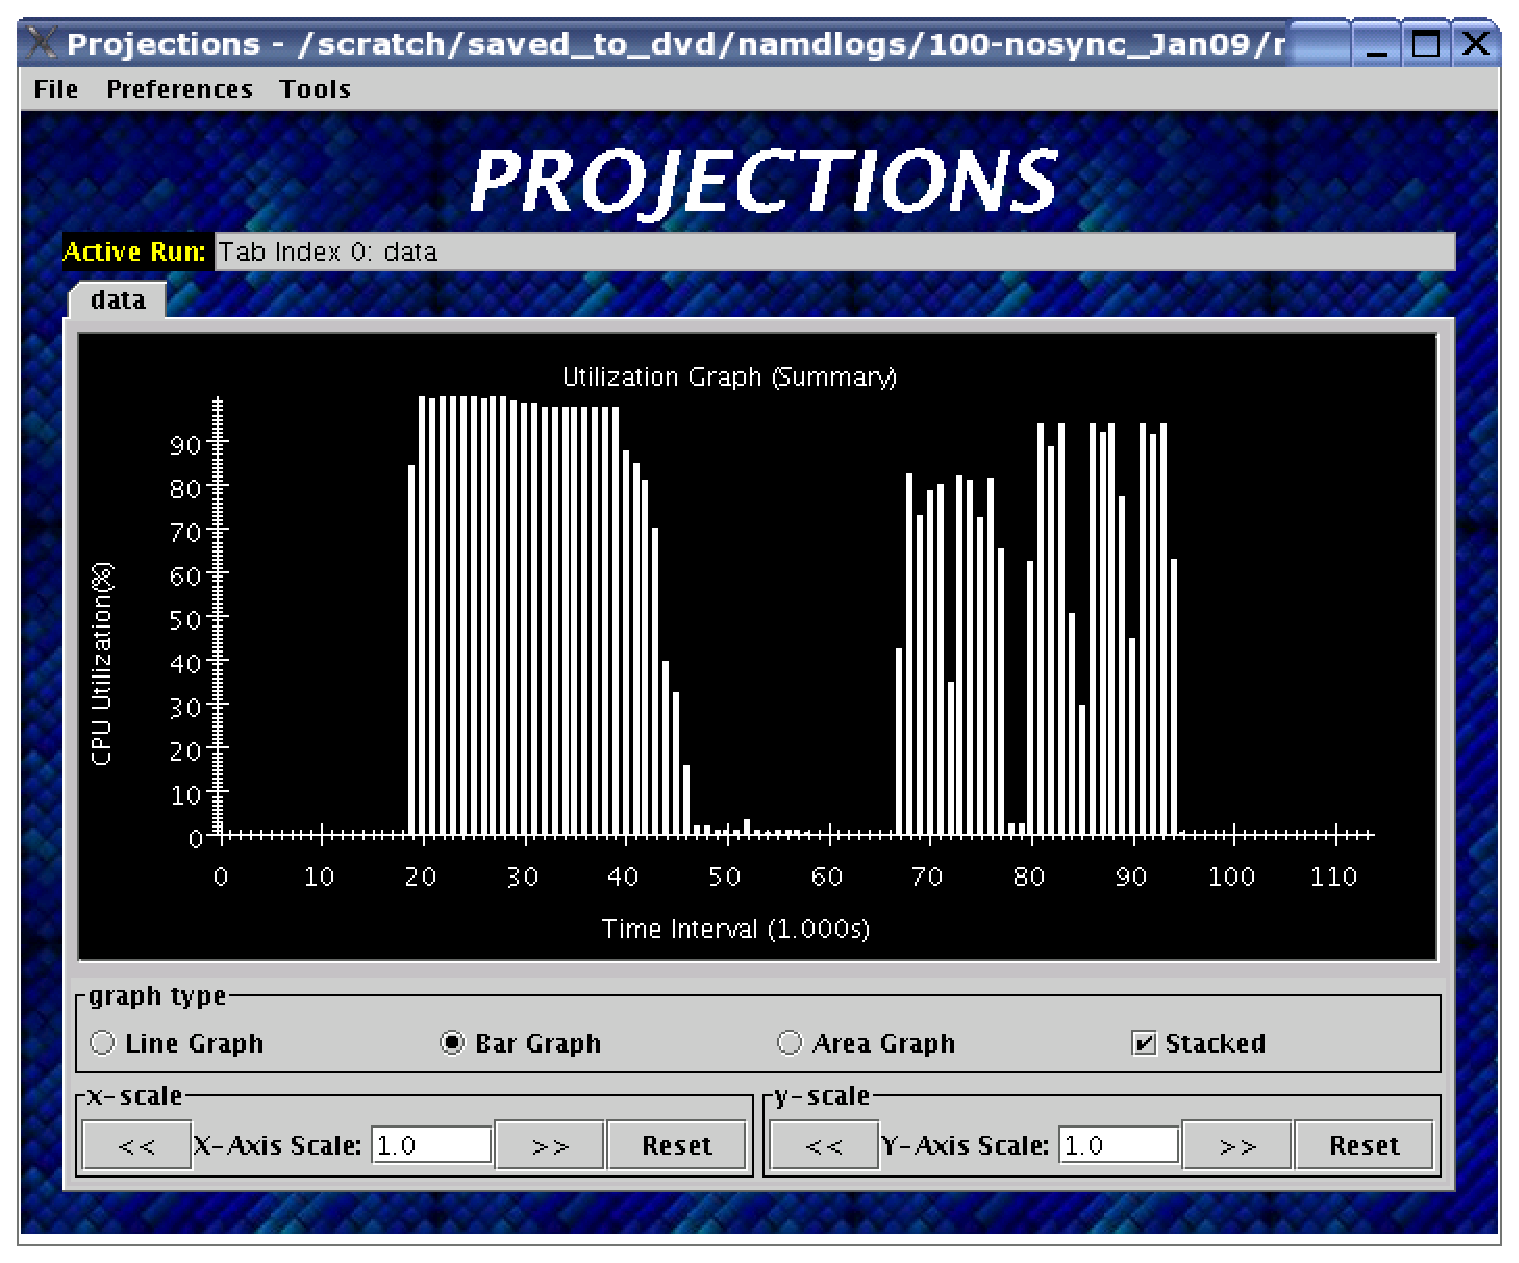
\includegraphics[width=4.0in]{fig/front-with-summary}
\caption{\projections{} main window}
\label{mainwindow}
\end{figure}

When \projections{} is started, it will display a main window as shown
in figure \ref{mainwindow}. If summary (.sum) files are available in
the set of data, a low-resolution utilization graph (Summary Display)
will be displayed as shown. If summary files are not available, or if
\projections{} was started without supplying the optional {\tt
NAME.sts} file, the main window will show a blank screen.

%{\bf Menu Options}

\begin{itemize}
\item
  {\bf File} contains 3 options. {\it Open File(s)} allows you to
  explicitly load a data set. This happens if you had not specified a
  {\tt NAME.sts} file in the command line when starting \projections{}
  or if you wish to explicitly load a new dataset. It brings up a
  dialog box that allows you to select the location of the dataset you
  wish to study. Navigate to the directory containing your data and
  select the .sts file.  Click on `Open'. If you have selected a valid
  file, \projections{} will load in some preliminary data from the
  files and then activate the rest of the options under the menu item
  {\bf Tools}. {\it Close current data} currently works the same way
  as {\it Close all data}. They unload all current \projections{} data
  so one can load in a new set of data. They will also deactivate the
  individual items provided in the {\bf Tools} menu option.
\item
  {\bf Preferences} generally allows you to set foreground or background
  colors and entry method color schemes. This is useful for configuring
  the color schemes of \projections{} windows to be print-friendly.
\item
  {\bf Tools} lists the set of available tools for analysis of generated
  trace data. It will be described in great detail under section
  \ref{sec::available tools}.
\end{itemize}

%{\bf Summary Display}

The Summary Display loaded on the Main Window displays basic processor
utilization data (averaged across all processors) over time
intervals. This is provided by the data generated by the summary
tracemode. This view offers no special features over and above the
{\bf Standard Graph Display} described in section \ref{sec::misc}. 
Please refer the appropriate section on information for using
its available features.

%{\bf Summary Display Performance Issues}

There should not be any serious performance issues involved in the
loading of summary data on the main window.

\subsection{Available Tools}
\label{sec::available tools}

The following tools and views become available to you after a dataset
has been loaded (with the exception of Multirun Analysis) and may be
accessed via the menu item Tools:

\begin{itemize}
\item 
The {\bf Graphs} view is where you can analyze your data by breaking it
into any number of intervals and look at what goes on in each of those
intervals.
\item
The {\bf Timelines} view lets you look at what a specific processor is
doing at each moment of the program. It is the most detailed view of a
parallel application \projections{} offers (and correspondingly, the
most resource-hungry).
\item
The {\bf Usage Profile} view lets you see percentage-wise what entry
methods each processor spends its time on during a specified time range.
It is particularly useful for identifying load imbalance and the probable
offending entry method.
\item
The {\bf Communication} view is a general tool that presents
communication properties contributed by each entry point across the
processors.
\item
The {\bf Log File Viewer} provides a human-readable, verbose
interpretation of a log file's entries.
\item
The {\bf Histograms} view presents entry point or communication
histogram information (ie. the frequency of occurrence of events given
an activity property like time bin size or message size on the
x-axis).
\item
The {\bf Overview} view gives user an overview of the utilization of
all processors during the execution. It is an extremely useful initial
tool to begin your performance analysis efforts with as it provides an
overall picture of application performance while being very
light-weight at the same time.
\item
The {\bf Animation} view animates the processor usage over a specified
range of time and a specified interval size.
\item
The {\bf Time Profile Graph} view is a more detailed presentation of
the {\bf Graphs} utilization view in that it presents the time
contribution by each entry point across the desired time
interval. While the {\bf Graphs} view can show the same data, it is
unable to stack the entry points, which proves useful in some cases.
\end{itemize}

\section{Performance Views}

\subsection{Graphs}
\label{sec::graph view}

%{\bf Introduction}

The Graphs window (see figure \ref{graph}) is where you can analyze your data by breaking it
into any number of intervals and look at what goes on in each of those
intervals.

%{\bf Dialog Box}

When the Graph Window first appears, a dialog box will also appear. It
will ask for the following information (Please refer to
\ref{sec::misc} for information on special features you can
use involving the various fields)::

\begin{itemize}
\item
Processor(s): Choose which processor(s) you wish to visualize graph 
information for.
\item
Start Time : Choose the starting time of interest. A time-based field.
\item
End Time : Choose the ending time of interest. A time-based field.
\item
Interval Size : Determine the size of an interval. The number of intervals
will also be determined by this value (End Time - Start Time divided by
Interval Size). A time-based field.
\end{itemize}

Standard \projections{} dialog options and buttons are also available
(see \ref{sec::misc} for details).

The following menu items are available:

\begin{itemize}
\item
{\bf File} contains 2 options: {\it Print Graph} uses Java's built-in 
print manager feature to render the tool's displays (usually to a printer 
or a file depending on the platform on which Java is supported). Note that
the current implementation of the renderer does not behave in exactly the
same fashion as the screen renderer, so you should expect the output to look
somewhat different. {\it Close} simply closes the Graph window.
\item
{\bf Tools} contains 2 options: {\it Set Interval Size} reloads the dialog
box so you could select a new time range over which to view Graph data.
{\it Timeline} is currently not implemented. Its intended as a convenient
way to load Timeline data (see section \ref{sec::timeline view}) over the 
same parameters as the current Graph view.
\end{itemize}

%{\bf Tool Performance }

The amount of time to analyze your data depends on several factors,
including the number of processors, number of entries, and number of
intervals you have selected.  A progress meter will show the amount of
data loaded so far. The meter will not, however, report rendering
progress which is determined mainly by the number of intervals selected.
As a rule of thumb, limit the number of intervals to 1,000 or less.

\begin{figure}[hbt]
\center
%\epsfig{figure=fig/graph.eps,height=4.3in}
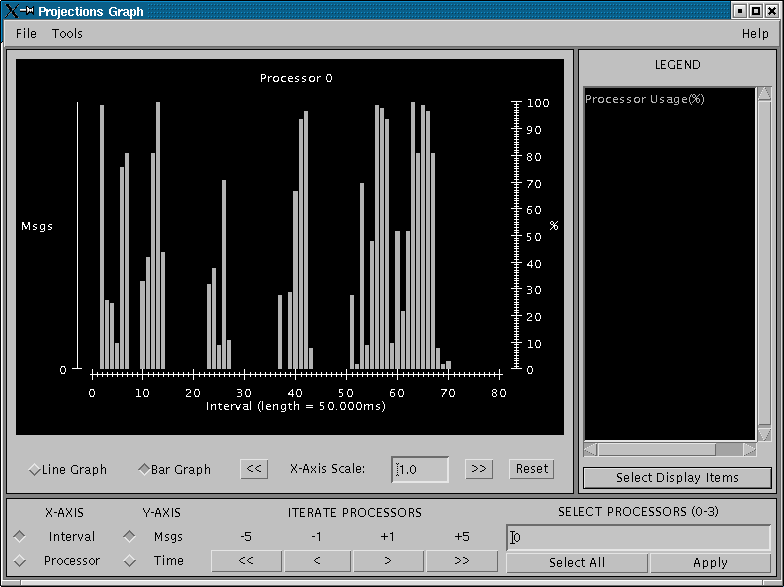
\includegraphics[width=4.3in]{fig/graph}
\caption{Graph tool}
\label{graph}
\end{figure}

%{\bf Tool Features }

The Graph Window has 3 components in its display:
\begin{enumerate}
\item[1)]
{\bf Display Panel} (located : top-left area)
   \begin{itemize}
   \item[-]
   Displays title, graph, and axes. To the left is a y-axis bar for
   detailed information involving the number of messages sent or time
   executed depending on the {\bf Control Panel} toggle selected (see 
   below). To the right is a y-axis bar for average processor-utilization 
   information. The x-axis may be based on time-interval or per-processor
   information depending on the appropriate {\bf Control Panel} toggle.
   \item[-]
   Allows you to toggle display between a line graph and a bar graph.
   \item[-]
   Allows you to scale the graph along the X-axis.  You can either
   enter a scale value $>=$ 1.0 in the text box, or you can use the
   $<<$ and $>>$ buttons to increment/decrement the scale by .25.
   Clicking on Reset sets the scale back to 1.0.  When the scale is
   greater than 1.0, a scrollbar will appear along the bottom of the
   graph to let you scroll back and forth.
   \end{itemize}
\item[2)]
{\bf Legend Panel} (located : top-right area)
   \begin{itemize}
   \item[-]
   Shows what information is currently being displayed on the graph and 
   what color represents that information.
   \item[-]
   Click on the `Select Display Items' button to bring up a window to
   add/remove items from the graph and to change the colors of the items:
      \begin{itemize}
      \item[*]
      The {\bf Select Display Items} window shows a list of items that you
      can display on the graph.  There are 3 main sections: System
      Usage, System Msgs, and User Entries. The System Usage and System
      Msgs are the same for all programs. The User Entries section
      has program-specific items in it.
      \item[*]
      Click on the checkbox next to an item to have it displayed on the
      graph.
      \item[*]
      Click on the colorbox next to an item to modify its color.
      \item[*]
      Click on `Select All' to choose all of the items
      \item[*]
      Click on `Clear All' to remove all of the items
      \item[*]
      Click on `Apply' to apply you choices/changes to the graph
      \item[*]
      Click on `Close' to exit
      \end{itemize}
   \end{itemize}
\item[3)]
{\bf Control Panel} (located : bottom area)
   \begin{itemize}
   \item[-]
   Allows you to toggle what is displayed on the X-axis.  You can either
   have the x-axis display the data by interval or by processor.
   \item[-]
   Allows you to toggle what is displayed on the Y-axis.  You can
   either have the y-axis display the data by the number of msgs sent
   or by the amount of time taken.
   \item[-]
   Allows you to change what data is being displayed by iterating
   through the selections.  If you have selected an x-axis type of
   `interval', that means you are looking at what goes on in each
   interval for a specific processor.  Clicking on the $<<, <, >, >>$
   buttons will change the processor you are looking at by either -5,
   -1, +1, or +5.  Conversely, if you have an x-axis of `processor',
   then the iterate buttons will change the value of the interval that
   you are looking at for each processor.
   \item[-]
   Allows you to indicate which intervals/processors you want to
   examine.  Instead of just looking at one processor or one interval,
   the box and buttons on the right side of this panel let you choose
   any number or processors/intervals to look at. This field behaves
   like a processor field. Please refer to section \ref{sec::misc} 
   for more information about the special features on using processor
   fields.

   Clicking on `Apply' updates the graph with your choices. Clicking
   on `Select All' chooses the entire processor range.  When you
   select more than one processor's worth of data to display, the
   graph will show the desired information summed across all selected
   processors. The exception to this is processor utilization data
   which is always displayed as data averaged across all selected
   processors.
   \end{itemize}
\end{enumerate}

\subsection{Timelines}
\label{sec::timeline view}

%{\bf Introduction}

The Timeline window (see figure \ref{timeline}) lets you look at what
a specific processor is doing at each moment of the program.

\begin{figure}[htb]
\center
%\epsfig{figure=fig/timeline.eps,height=3.8in}
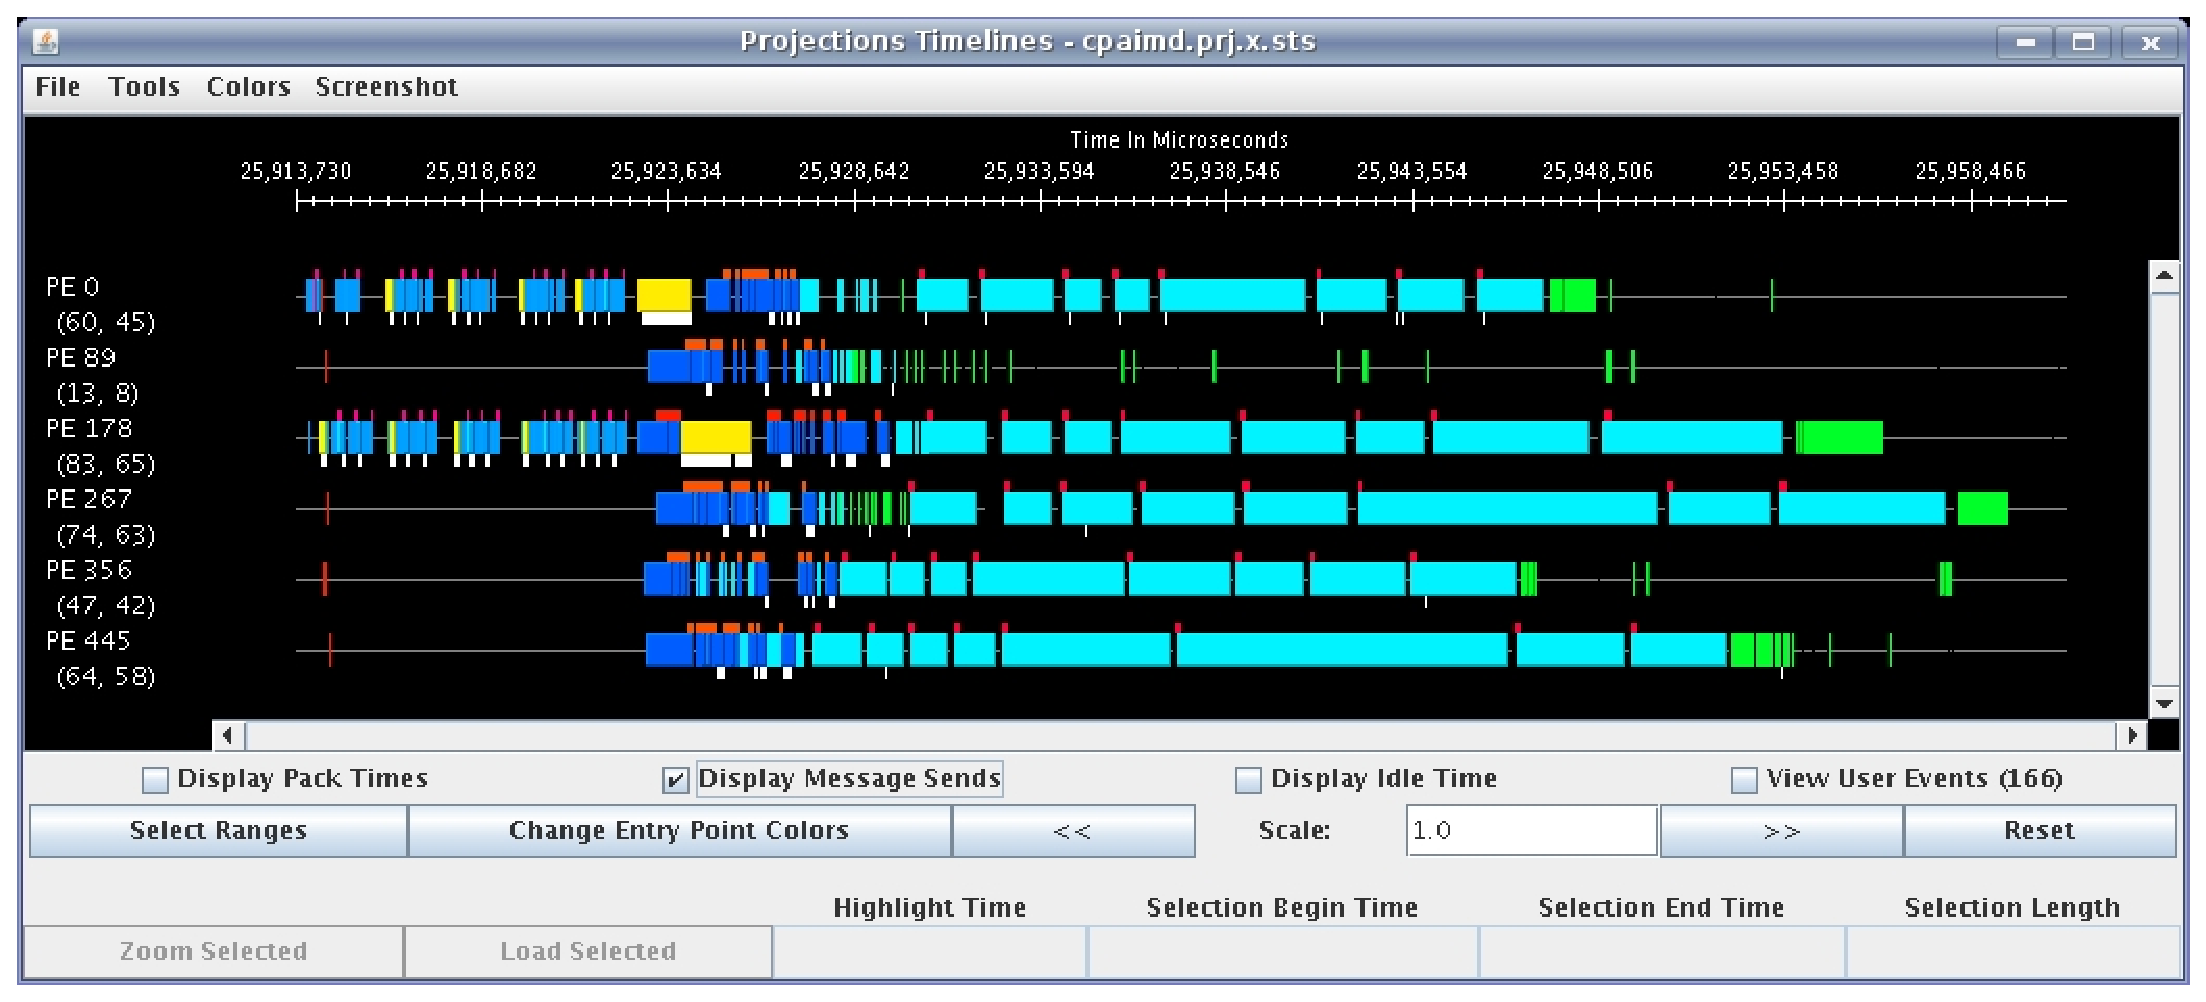
\includegraphics[width=3.8in]{fig/timeline}
\caption{Timeline Tool}
\label{timeline}
\end{figure}

%{\bf Dialog Box}

When opening a Timeline view, a dialog box appears. 
The box asks for the following information (Please refer to
\ref{sec::misc} for information on special features you can
use involving the various fields):

\begin{itemize}
\item
Processor(s): Choose which processor(s) you want to see in the timeline.
\item
Start Time  : Choose what time you want your timeline to start at.
A time-based field.
\item
End Time    : Choose what time you want your timeline to end at. A time-based
field.
\end{itemize}

Standard \projections{} dialog options and buttons are also available
(see \ref{sec::misc} for details).


The following menu options are available:

\begin{itemize}
\item {\bf File} contains 1 enabled option: 
{\it Close} simply closes the Timeline Window.
\item {\bf Tools} contains 1 option: {\it Modify Ranges} opens the initial 
dialog box thereby allowing you to select new set of processors or time duration
parameters.
\item {\bf Colors} contains options for loading, using, and modifying color schemes. {\it Change Colors} functions in
a manner similar to the button of the same name described under control 
panel information below. {\it Save Colors} allows you to save the current
color set to a file named ``color.map'' into the same directory where your
data logs are stored. Note that the directory must have write permissions
for you before this can work. We are currently working on a more flexible
scheme for storing saved color sets. {\it Restore Colors} allows you to
load any previously saved color sets described above. {\it Default Colors}
resets the current color set to the default set that \projections{} assigns
without user intervention.

Other color schemes are provided that can be used for some applications. The colors set as described above are the default coloring scheme. Other options for coloring the events are by event id (chare array index), user supplied parameter, or memory usage. In order to color by a user supplied parameter such as timestep, the C function  \texttt{traceUserSuppliedData(int value);} should be called within some entry methods. If such a method is called in an entry method, the entry method invocation can be colored by the parameter. The user supplied data can also be viewed in the tooltip that appears when the cursor hovers over an entry method invocation in the window. To color by memory usage, the C function \texttt{traceMemoryUsage();} should be called in all entry methods. The call records the current memory usage. Red indicates high memory usage, and green indicates low memory usage. The actual memory usage can also be viewed in the tooltips that appear when the cursor is over an event. The memory usage is only available in when using a Charm++ version that uses gnu memory.


\item {\bf Screenshot} contains 1 option: 
{\it Save as JPG or PNG} save the visible portion of the visualization
to an image file. You must choose a filename ending with a \texttt{.png}
or \texttt{.jpg} extension when choosing the location to save the image. The
appropriate filetype is chosen based on the chosen filename
extension. If the view is zoomed in, only the portion currently shown
on screen is saved.

\end{itemize}

The Timeline Window consists of two parts:
\begin{enumerate}
\item[1)]
{\bf Display Panel} (located: top area)

This is where the timelines are displayed and is the largest portion
of the window.  The time axis is displayed at the top 
of the panel.  The left side of the
panel shows the processor labels, each containing a processor number and
two strange numbers. These two numbers represent the percentage of the
loaded timeline during which work occurs. The first of the two numbers
is the ``non-idle'' time, i.e. the portion of the time in the timeline
not spent in idle regions. This contains both time for entry methods
as well as other uninstrumented time spent likely in the Charm++
runtime. The second number is the percentage of the time used by the
entry methods for the selected range.


The timeline itself consists of colored bars for each event.
Placing the cursor over any of these bars will display information 
about the event including:  the name, the begin time, the end
time, the total time, the time spent packing, the number of messages it
created, and which processor created the event. 

Left clicking on an event bar will cause a window to popup. This
window contains detailed information about the messages sent by the
clicked upon event.

Right clicking on an event bar will cause a line to be drawn to the
beginning of the event bar from the point where the message causing
the event originated. This option may not be applicable for threaded
events. If the message originated on a processor not currently
included in the visualization, the other processor will be loaded, and
then the message line will be drawn. A warning message will appear if
the message origination point is outside the time duration, and hence
no line will be drawn.

User events are displayed as bars above the ordinary
event bars in the display area. If the name of the user event contains a substring ``***'' then the bar will vertically span the whole screen.

Message pack times and send points can be displayed below the event
bars. The message sends are small white tick marks, while the message
pack times are small pink bars usually occurring immediately after the
message send point. If zoomed in to a point where each microsecond
takes more than one pixel, the message send point and the following
packing time may appear disconnected. This is an inherent problem with
the granularity used for the logfiles.


\item[2)]
{\bf Control Panel} (located: bottom area)

The controls in this panel are obvious, but we mention one here anyway.

   View User Event - Checking this box will bring up a new
   window showing the string description, begin time, end time and
   duration of all user events on each processor. You can access
   information on user events on different processors by accessing the
   numbered tabs near the top of the display.

   \begin{figure}[htb]
   \center
%\epsfig{figure=fig/userevent.eps,height=1.5in}
   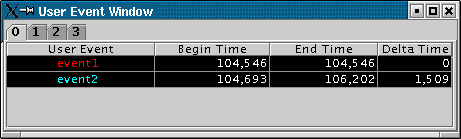
\includegraphics[height=1.5in]{fig/userevent}
   \caption{User Event Window}
   \label{userevent}
   \end{figure}

\end{enumerate}

Various features appear when the user moves the mouse cursor over the
top axis. A vertical line will appear to highlight a specific
time. The exact time will be displayed at the bottom of the
window. Additionally a user can select a range by clicking while a
time is highlighted and dragging to the left or right of that
point. As a selection is being made, a vertical white line will mark
the beginning and end of the range. Between these lines, the
background color for the display will change to gray to better
distinguish the selection from the surrounding areas. After a
selection is made, its duration is displayed at the bottom. A user can
zoom into the selection by clicking the ``Zoom Selected'' button. To
release a selection, single-click anywhere along the axis. Clicking
``Load Selected'' when a selection is active will cause the timeline
range to be reloaded. To zoom out, the ``<<'' or ``Reset'' button can be used.


To then zoom into the selected area via this interface, click on
either the ``Zoom Selected'' or the ``Load Selected'' buttons.  The
difference between these two buttons is that the "Load Selected" zooms
into the selected area and discards any events that are outside the
time range.  This is more efficient than ``Zoom Selected'' as the
latter draws all the events on a virtual canvas and then zooms into
the canvas. The disadvantage of using ``Load Selected'' is that it
becomes impossible to zoom back out without having to re-specify the
time range via the ``Select Ranges'' button.

Performance-wise, this is the most memory-intensive part of the
visualization tool. The load and zoom times are proportional to the
number of events displayed. The user should be aware of how event-intensive the application is
over the desired time-period before proceeding to use this view. If
\projections{} takes too long to load a timeline, cancel the load and
choose a smaller time range or fewer processors. We expect to add features to alleviate
this problem in future releases.

\subsection{Usage Profile}
\label{sec::usage profile}
The Usage Profile window (see figure \ref{usage profile}) lets you see
percentage-wise what each processor spends its time on during a
specified period.

When the window first comes up, a dialog box appears asking for the
processor(s) you want to look at as well as the time range you want to
look at.  This dialog functions in exactly the same way as for the Timeline
tool (see section \ref{sec::timeline view}).

\begin{figure}[htb]
\center
%\epsfig{figure=fig/usageprofile.eps,height=4in}
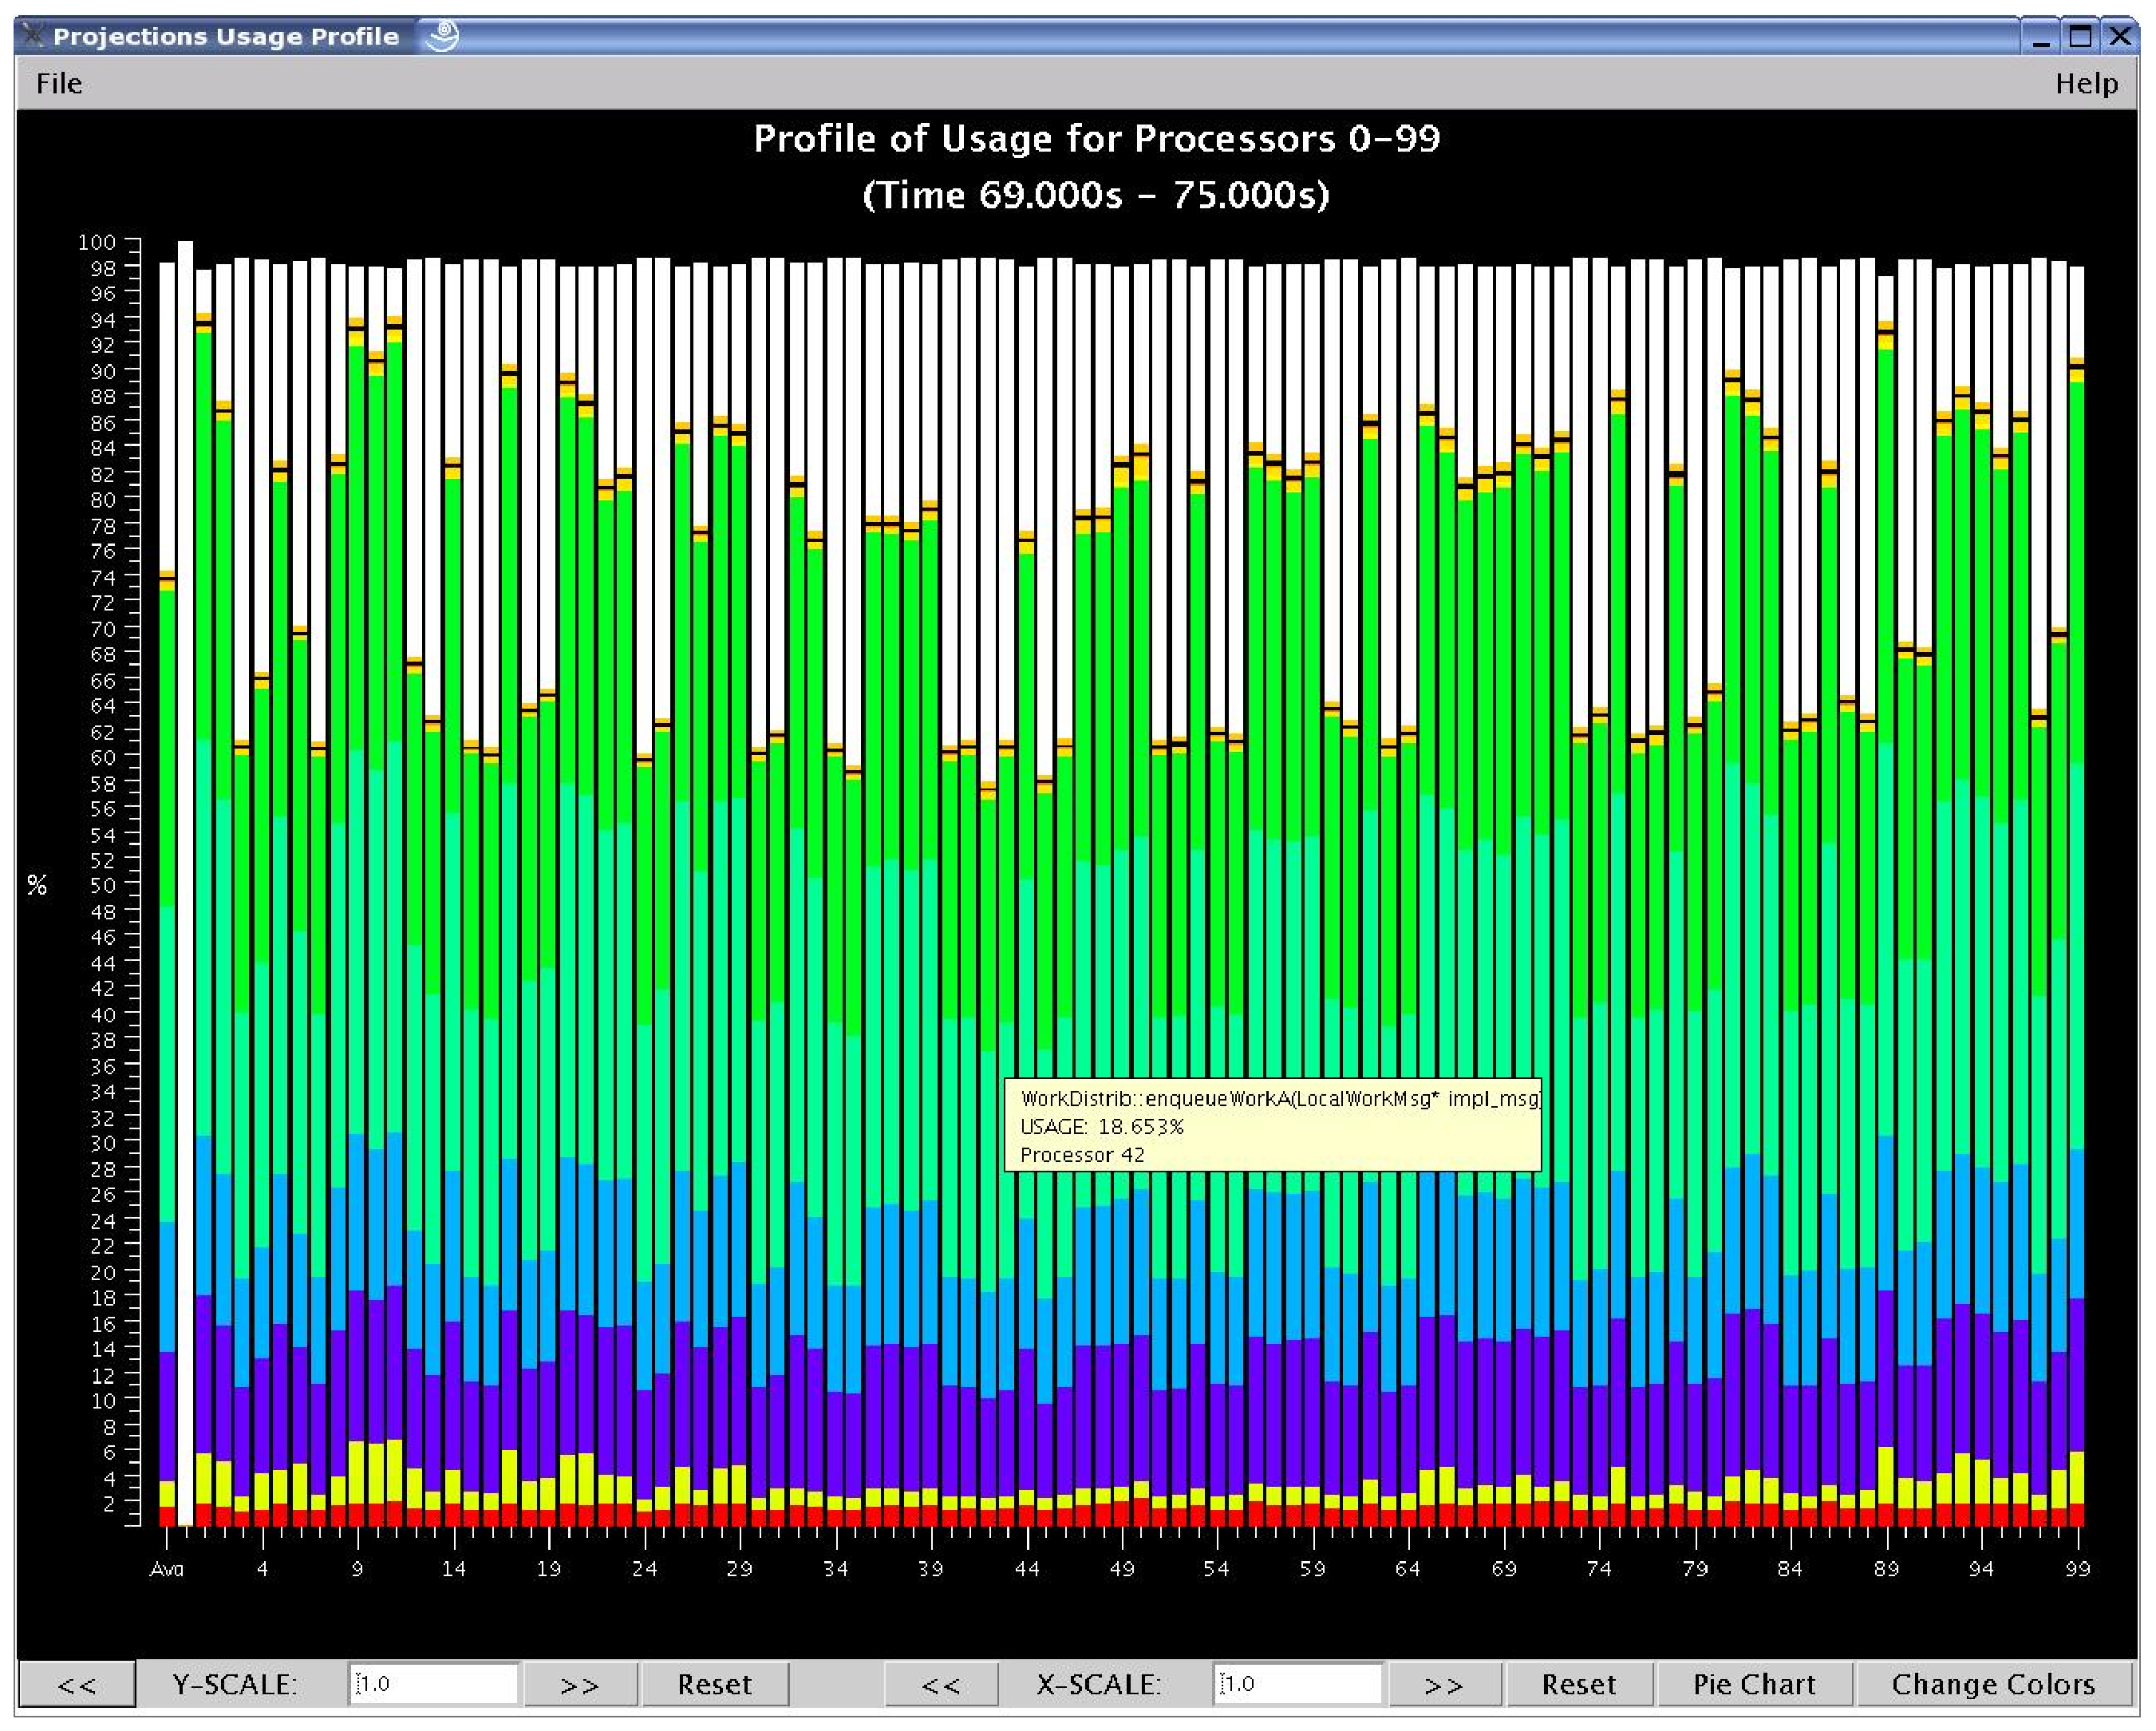
\includegraphics[width=4.0in]{fig/usageprofile}
\caption{Usage Profile}
\label{usage profile}
\end{figure}

The following menu options are available in this view:

\begin{itemize}
\item {\bf File} has 2 options: {\it Select Processors} reloads the dialog
box for the view and allows you to select a new processor and time range
for this view. {\it Print Profile} currently does nothing. This will be
addressed in a later release of \projections{}.
\end{itemize}

The following components are supported in this view:

\begin{itemize}
\item[1)] 
{\bf Main Display} (located: top area) 
The left axis of the display shows a scale from 0\% to 100\%.  The
main part of the display shows the statistics.  Each processor is
represented by a vertical bar with the leftmost bar representing the
statistics averaged across all processors. The bottom of the bar
always shows the time spent in each entry method (distinguished by the
entry method's assigned color) . Above that is always reported the
message pack time (in black), message unpack time (in orange) and idle
time (in white). Above this, if the information exists, are colored
bars representing communication CPU overheads contributed by each
entry method (again, distinguished by the same set of colors
representing entry methods). Finally the black area on top represents
time overheads that the \charmpp{} runtime cannot account for.

If you mouse-over a portion of the bar (with the exception of the
black area on top), a pop-up window will appear telling you the name
of the item, what percent of the usage it has, and the processor it is
on.

\item[2)]
{\bf Control Panel} (located: bottom area)
The panellets you adjust the scales in both the X and Y directions.
The X direction is useful if you are looking at a large number of
processors. The Y direction is useful if there are small-percentage
items for a processor. The ``Reset'' button allows you to reset the 
X and Y scales.

The ``Pie Chart'' button generates a pie chart representation (see
figure \ref{piechart}) of the same information using averaged
statistics but without idle time and communication CPU overheads.

\begin{figure}[htb]
\center
%\epsfig{figure=fig/piechart.eps,height=1in}
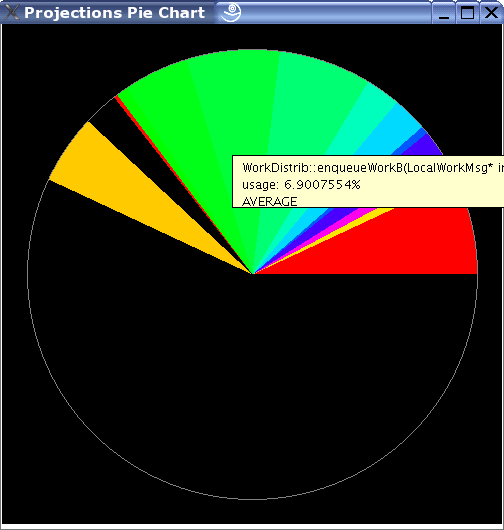
\includegraphics[width=1.8in]{fig/piechart}
\caption{Pie Chart representation of average usage}
\label{piechart}
\end{figure}

The ``Change Colors'' button lists all entry methods displayed on the
main display and their assigned colors. It allows you to change those
assigned colors to aid in highlighting entry methods.

The resource consumption of this view is moderate. Load times and
visualization times should be relatively fast, but dismissing the tool
may result in a very slight delay while \projections{} reclaims memory
through Java's garbage collection system.

\end{itemize}

\subsection{Communication}
\label{sec::communication}

The communication tool (see figure \ref{communication}) visualizes
communication properties on each processor over a user-specified time
range.

The dialog box of the tool allows you to specify the time period
within which to load communication characteristics information. This
dialog box is exactly the same as that of the Timeline tool (see
section \ref{sec::timeline view}).

The main component employs the standard capabilities provided by
\projections{}' standard graph (see \ref{sec::misc}).

The control panel allows you to switch between the following
communication characteristics:

\begin{itemize}
\item[-] Number of Messages Sent by entry methods (initial default view);
\item[-] Number of Bytes Sent by entry methods;
\item[-] Number of Messages Received by entry methods;
\item[-] Number of Bytes Received by entry methods;
\item[-] Number of Messages Sent externally (physically) by entry methods;
\item[-] Number of Bytes Sent externally (physically) by entry methods;
\item[-] and Number of hops messages travelled before being received
by an entry methods. This is available when the runtime option {\tt -bgsize}
(See section \ref{sec:startingUp}) is supplied.
\end{itemize}

\begin{figure}[htb]
\center
%\epsfig{figure=fig/commhistogram.eps,height=4in}
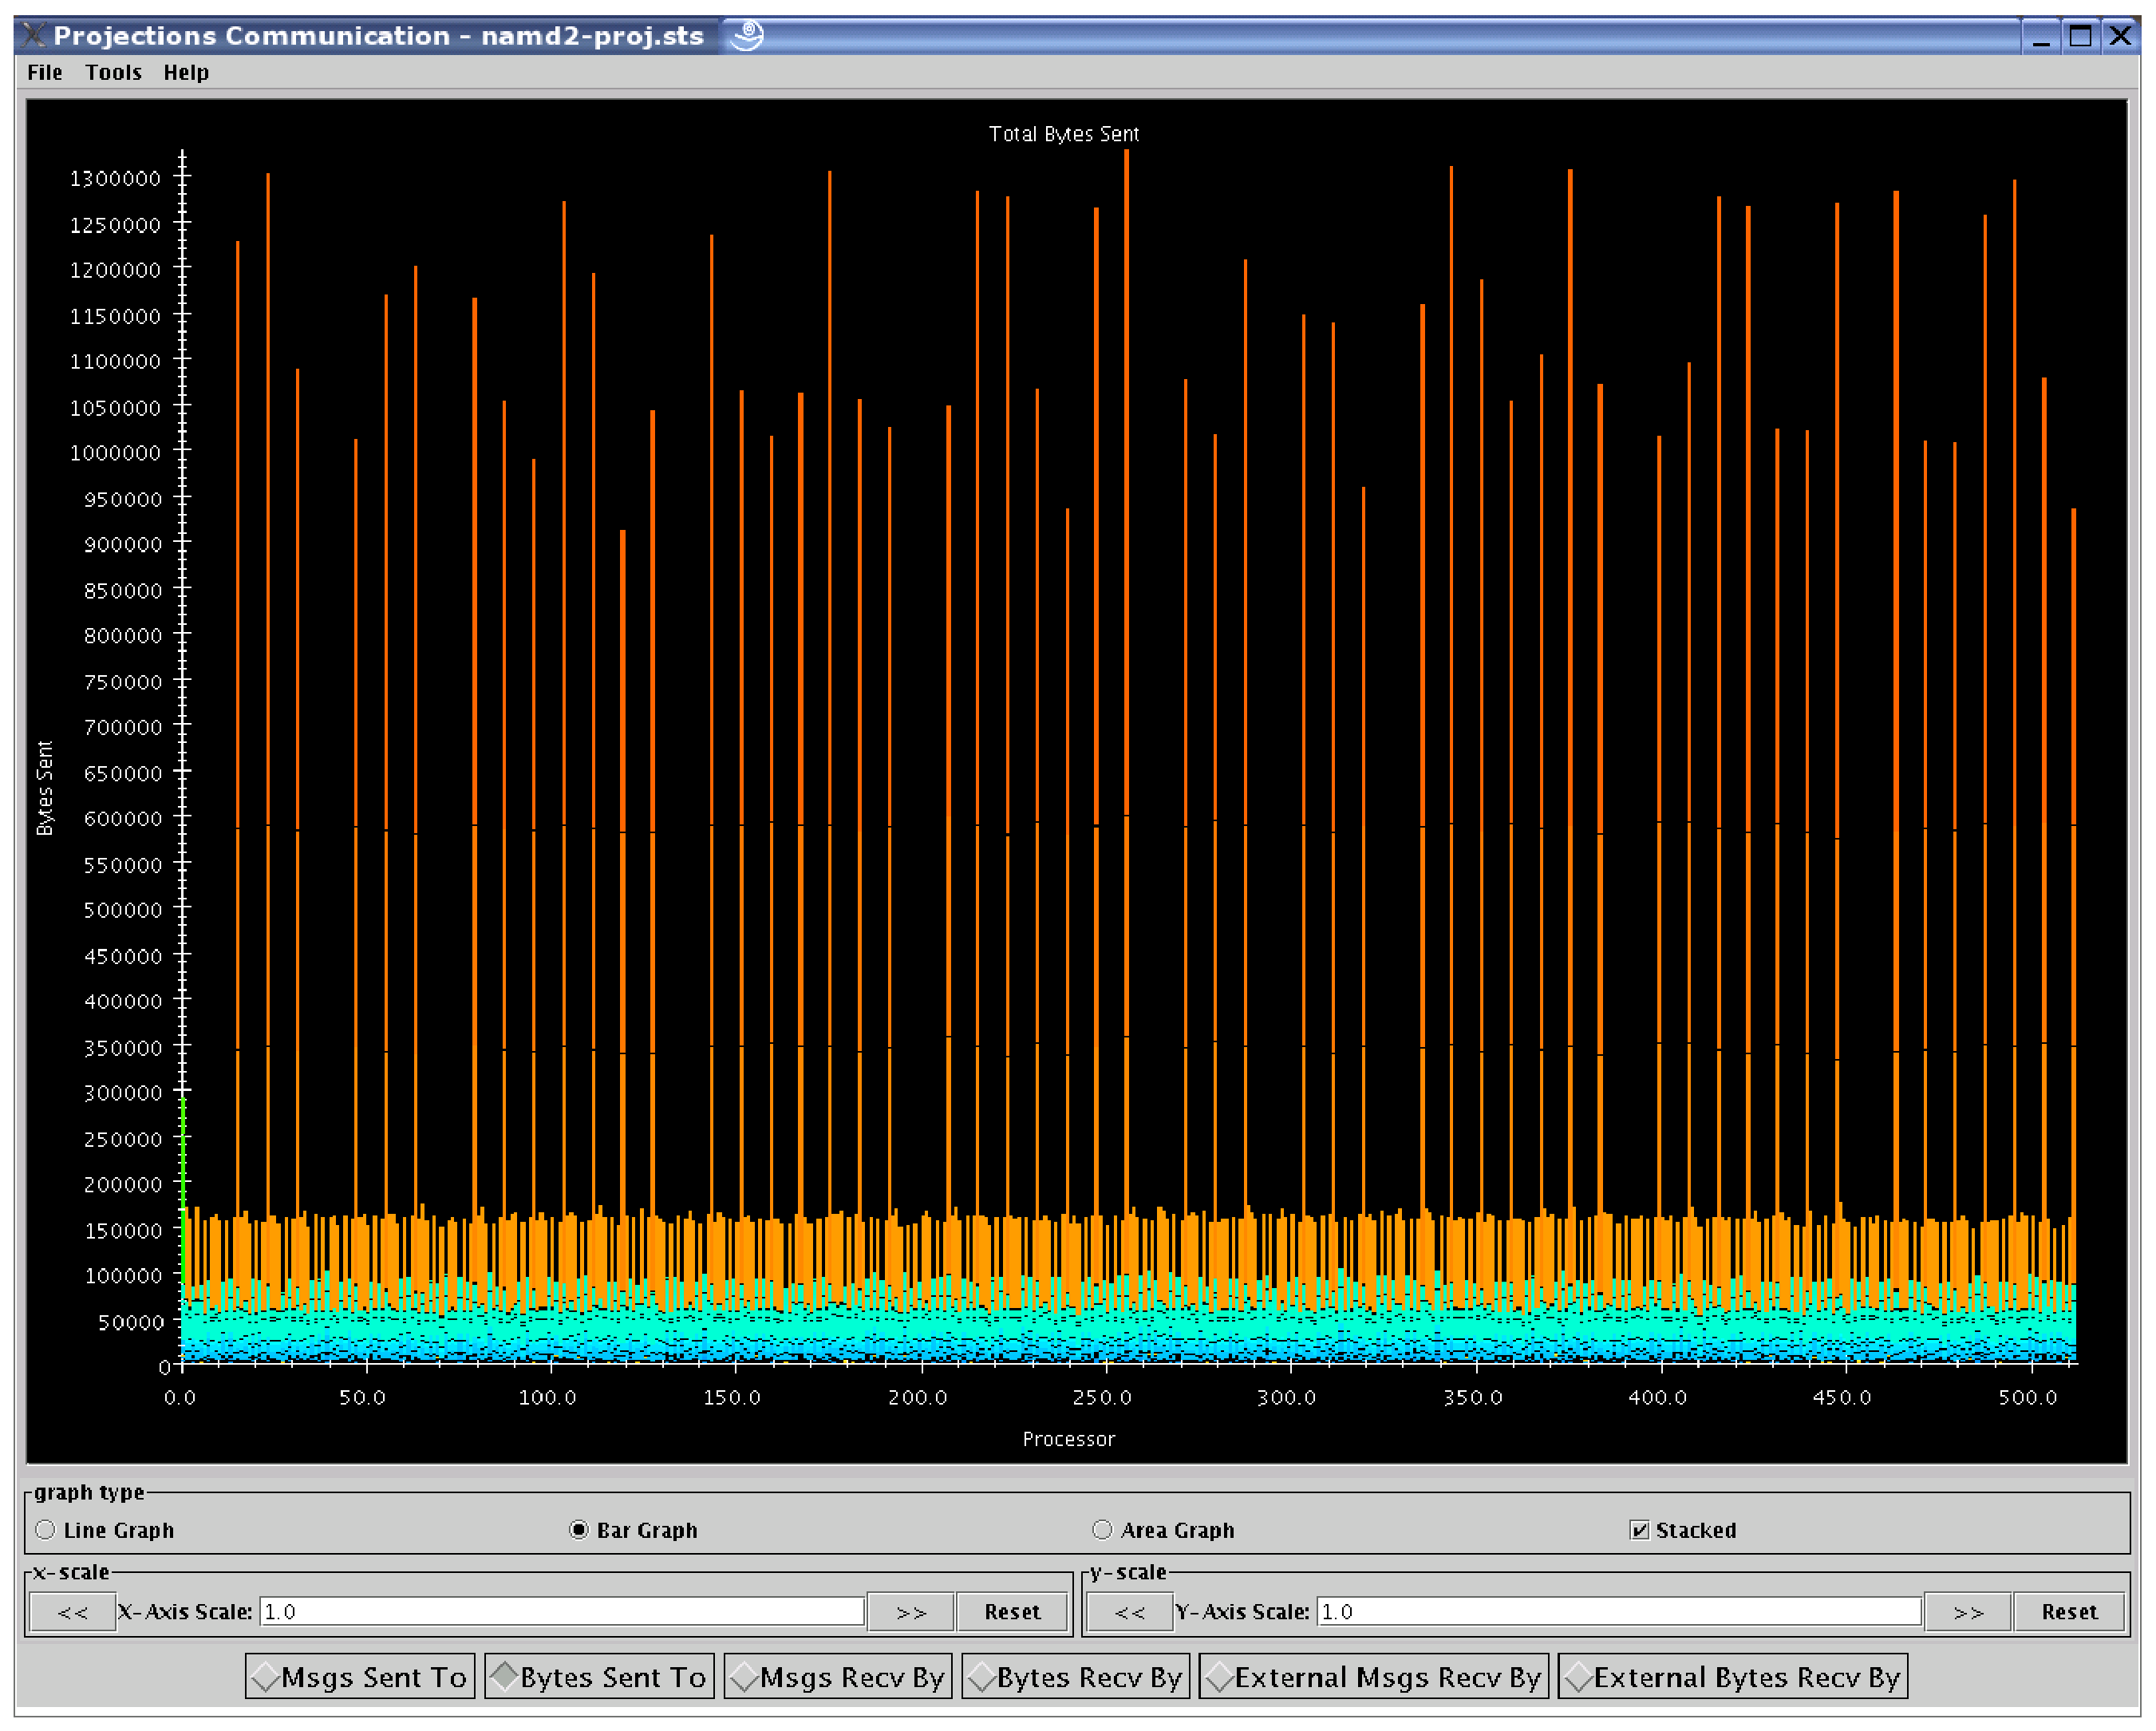
\includegraphics[width=4.0in]{fig/apoa1_512_CommProcessorProfile}
\caption{Communication View}
\label{communication}
\end{figure}

This view uses memory proportional to the number of processors selected.

\subsection{Communication vs Time}

The communication over time tool (see figure \ref{communication-time})
visualizes communication properties over all processors and displayed
over a user-specified time range on the x-axis.

The dialog box of the tool allows you to specify the time period
within which to load communication characteristics information. This
dialog box is exactly the same as that of the Communication tool (see
section \ref{sec::communication}).

The main component employs the standard capabilities provided by
\projections{}' standard graph (see \ref{sec::misc}).

The control panel allows you to switch between the following
communication characteristics:

\begin{itemize}
\item[-] Number of Messages Sent by entry methods (initial default view);
\item[-] Number of Bytes Sent by entry methods;
\item[-] Number of Messages Received by entry methods;
\item[-] Number of Bytes Received by entry methods;
\item[-] Number of Messages Sent externally (physically) by entry methods;
\item[-] Number of Bytes Sent externally (physically) by entry methods;
\item[-] and Number of hops messages travelled before being received
by an entry methods (available only on trace logs generated on the
Bluegene machine).
\end{itemize}

\begin{figure}[htb]
\center
%\epsfig{figure=fig/commhistogram.eps,height=4in}
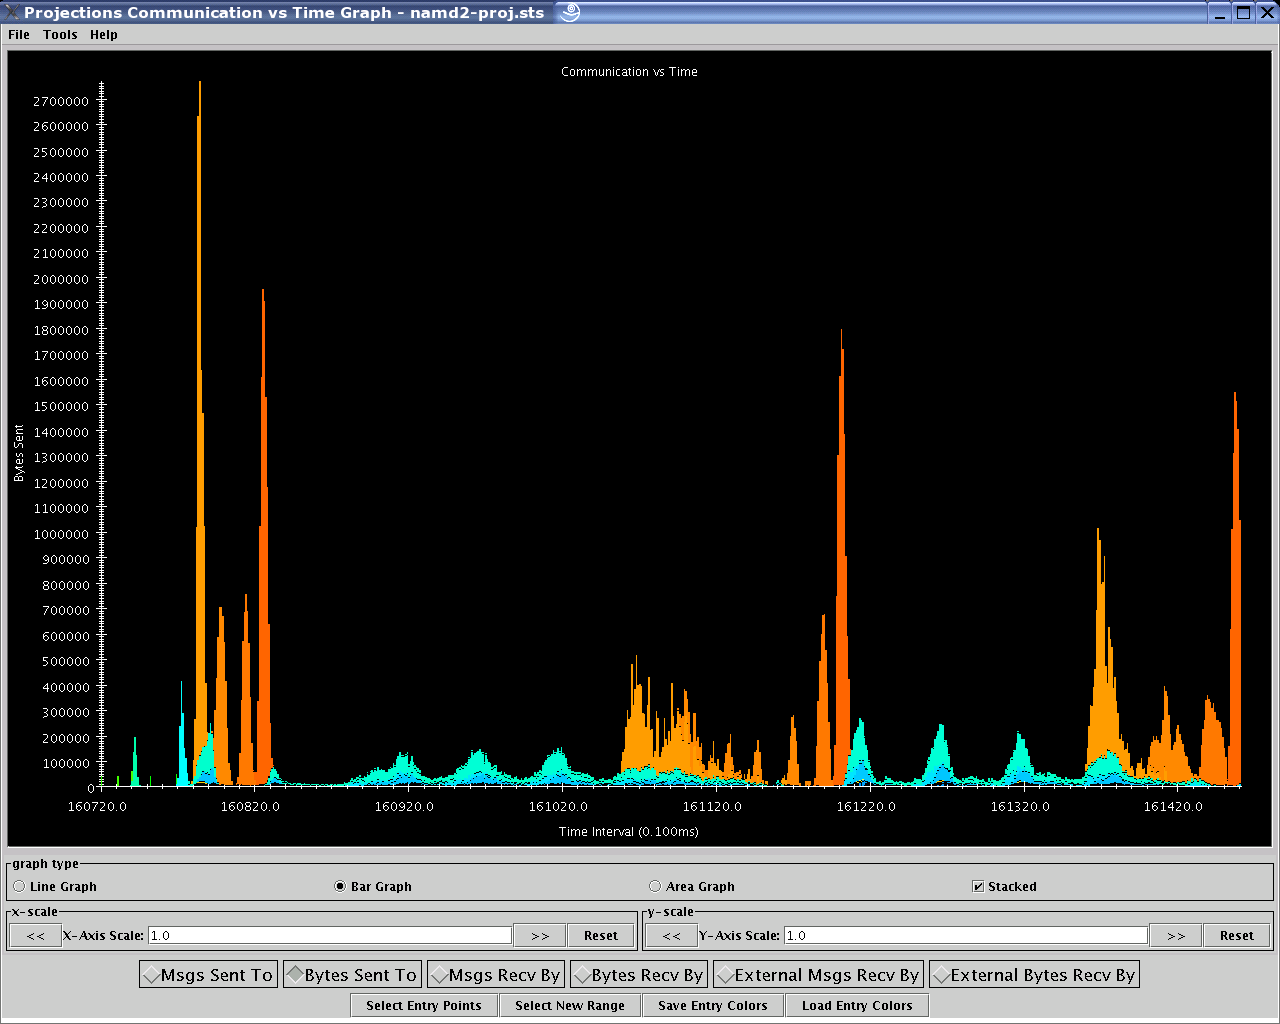
\includegraphics[width=4.0in]{fig/apoa1_512_CommTimeProfile}
\caption{Communication View over Time}
\label{communication-time}
\end{figure}

This view has no known problems loading any range or volume of data.

\subsection{View Log Files}

This window (see figure \ref{viewlog}) lets you see a translation of a
log file from a bunch of numbers to a verbose version.  A dialog box
asks which processor you want to look at.  After choosing and pressing
OK, the translated version appears. Note that this is {\it not} a
standard processor field. This tool will only load {\it exactly} one
processor's data.

\begin{figure}[htb]
\center
%\epsfig{figure=fig/viewlog.eps,height=4in}
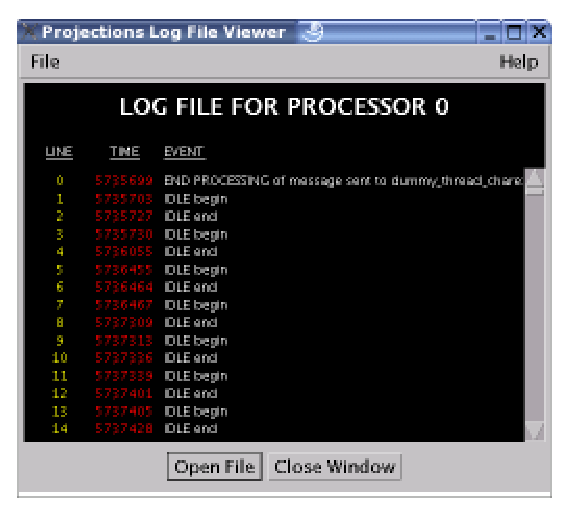
\includegraphics[width=2.5in]{fig/viewlog}
\caption{Log File View}
\label{viewlog}
\end{figure}

Each line has:
\begin{itemize}
\item[-] a line number (starting at 0)
\item[-] the time the event occurred at
\item[-] a description of what happened.
\end{itemize}

This tool has the following menu options:

\begin{itemize}
\item {\bf File} has 2 options: {\it Open File} reloads the dialog box
and allows the user to select a new processor's data to be loaded.
{\it Close} closes the current window.
\item {\bf Help} has 2 options: {\it Index} currently does not do anything.
This will be addressed in a later release of \projections{}. {\it About}
currently does not do anything. This will also be addressed in a later
release of \projections{}.
\end{itemize}

The tool has 2 buttons. ``Open File'' reloads the dialog box (described 
above) and allows the user to select a new processor's data to be loaded.
``Close Window'' closes the current window.

\subsection{Histograms}

This module (see figure \ref{histogram}) allows you to examine the
performance property distribution of all your entry points (EP). It
gives a histogram of different number of EP's that have the following
properties falling in different property bins:

The dialog box for this view asks the following information from the
user. (Please refer to \ref{sec::misc} for information on special
features you can use involving the various fields):

\begin{itemize}
\item
Processor(s): Choose which processor(s) you wish to visualize histogram
information for.
\item
Start Time: Choose the starting time of interest. A time-based field.
\item
End Time: Choose the ending time of interest. A time-based field.
\item
Number of Bins: Select the number of property bins to fit frequency data
under. A simple numeric field.
\item
Size of Bin: Determine (in units - microseconds or bytes) how large each
bin should be. A simple numeric field.
\item
Starting Bin Size: Determine (in units - microseconds or bytes) how
far to offset the data. This is useful for ignoring data that is too
small to be considered significant, but could overwhelm other data
because of the sheer numbers of occurrences. A simple numeric field.
\end{itemize}

The dialog box reports the selection of bins as specified by the user
by displaying the minimum bin size (in units - microseconds or bytes)
to the maximum bin size. ``units'' refer to microseconds for time-based
histograms or bytes for histograms representing message sizes.

Standard graph features can be employed for the main display of this
view (see section \ref{sec::misc}). 

The following menu items are available in this tool:

\begin{itemize}
\item {\bf File} offers 3 options: {\it Select Entry Points} currently
does nothing. It is intended to behave similarly to the button ``Select
Entries'' described below. This will be fixed in a later release of
\projections{}. {\it Set Range} reloads the dialog box and allows the
user to load data based on new parameters. {\it Close} closes the current
tool window.
\item {\bf View} provides 1 option: {\it Show Longest EPs} currently
does nothing. It is intended to behave similarly to the button 
``Out-of-Range EPs'' and will be fixed in a later release of \projections{}.
\end{itemize}

The following options are available in the control panel in the form
of toggle buttons:

\begin{itemize}
\item[-] Entry method execution time (How long did that entry method ran 
for?)
\item[-] Entry method creation message size (How large was the message
that caused the entry method's execution?)
\end{itemize}

\begin{figure}[htb]
\center
%\epsfig{figure=fig/histogram.eps,height=4in}
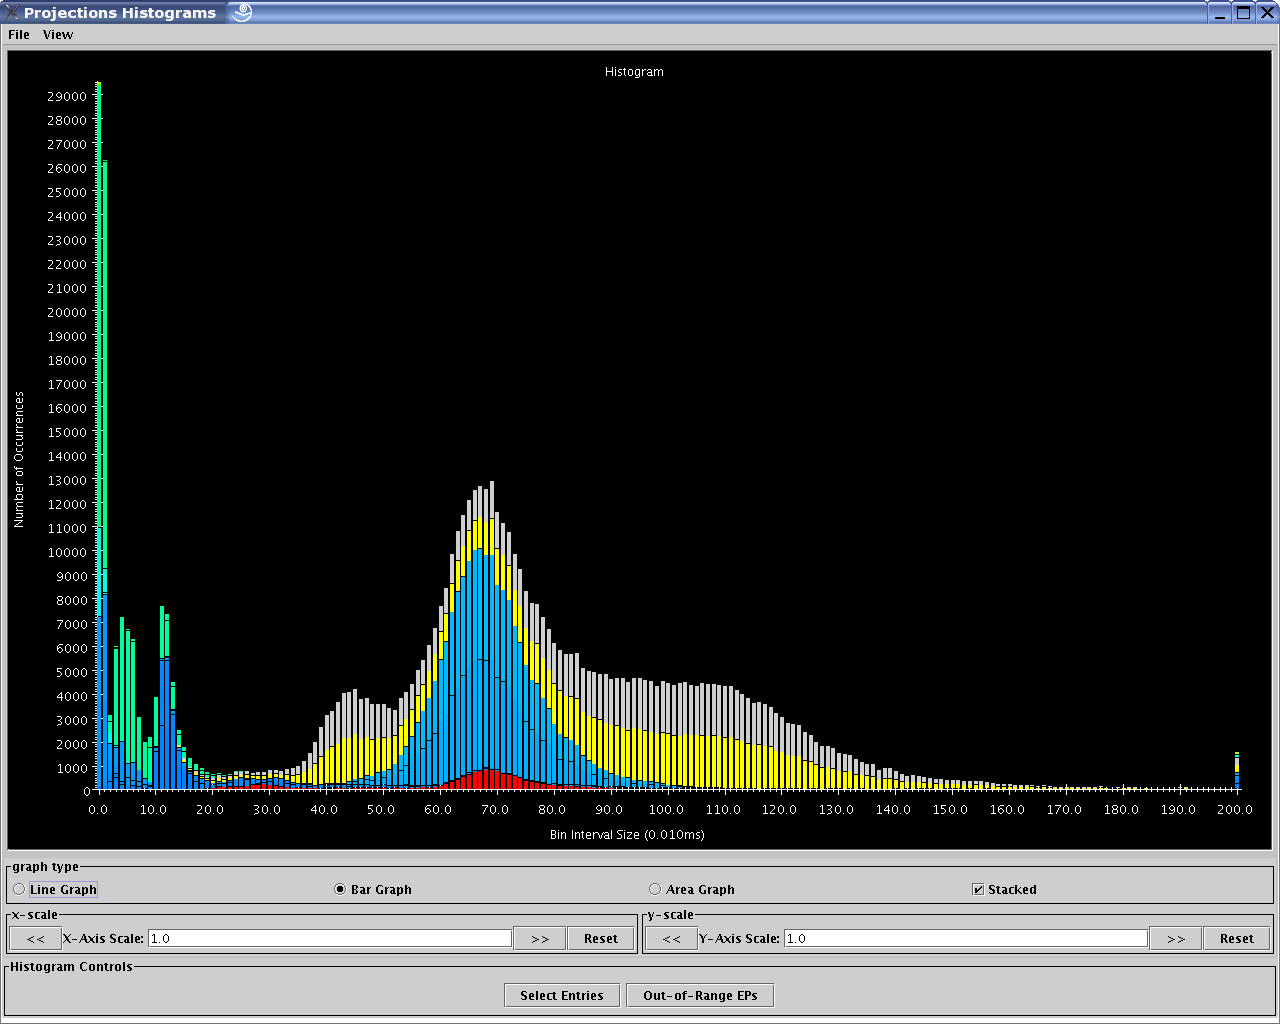
\includegraphics[width=4.0in]{fig/histogram}
\caption{Histogram view}
\label{histogram}
\end{figure}

The use of the tool is somewhat counterintuitive. The dialog box is
created immediately and when the tool window is created, it is
defaulted to a time-based histogram. You may change this histogram to
a message-size-based histogram by selecting the ``Message Size'' radio
button which would then update the graph using the same parameters
provided in the dialog box. This issue will be fixed in upcoming
editions of \projections{}.

The following features are, as of this writing, not implemented. They
will be ready in a later release of \projections{}.

The ``Select Entries'' button is intended to bring up a color
selection and filtering window that allows you to filter away entry
methods from the count. This offers more control over the analysis
(e.g. when you already know EP 5 takes 20-30ms and you want to know if
there are other entry points also takes 20-30ms).

The ``Out-of-Range EPs'' button is intended to bring up a table
detailing all the entry methods that fall into the overflow (last)
bin. This list will, by default, be listed in descending order of time
taken by the entry methods.

The performance of this view is affected by the number of bins the
user wishes to analyze. We recommend the user limits the analysis to
1,000 bins or less.

\subsection{Overview}

Overview (see figure \ref{overview}) gives users an overview of the
utilization of all processors during the execution over a
user-specified time range.

The dialog box of the tool allows you to specify the time period
within which to load overview information. This dialog box is exactly
the same as that of the Timeline tool (see section \ref{sec::timeline
view}).

\begin{figure}[!ht]
  \centering
  \subfigure[Overview]{
    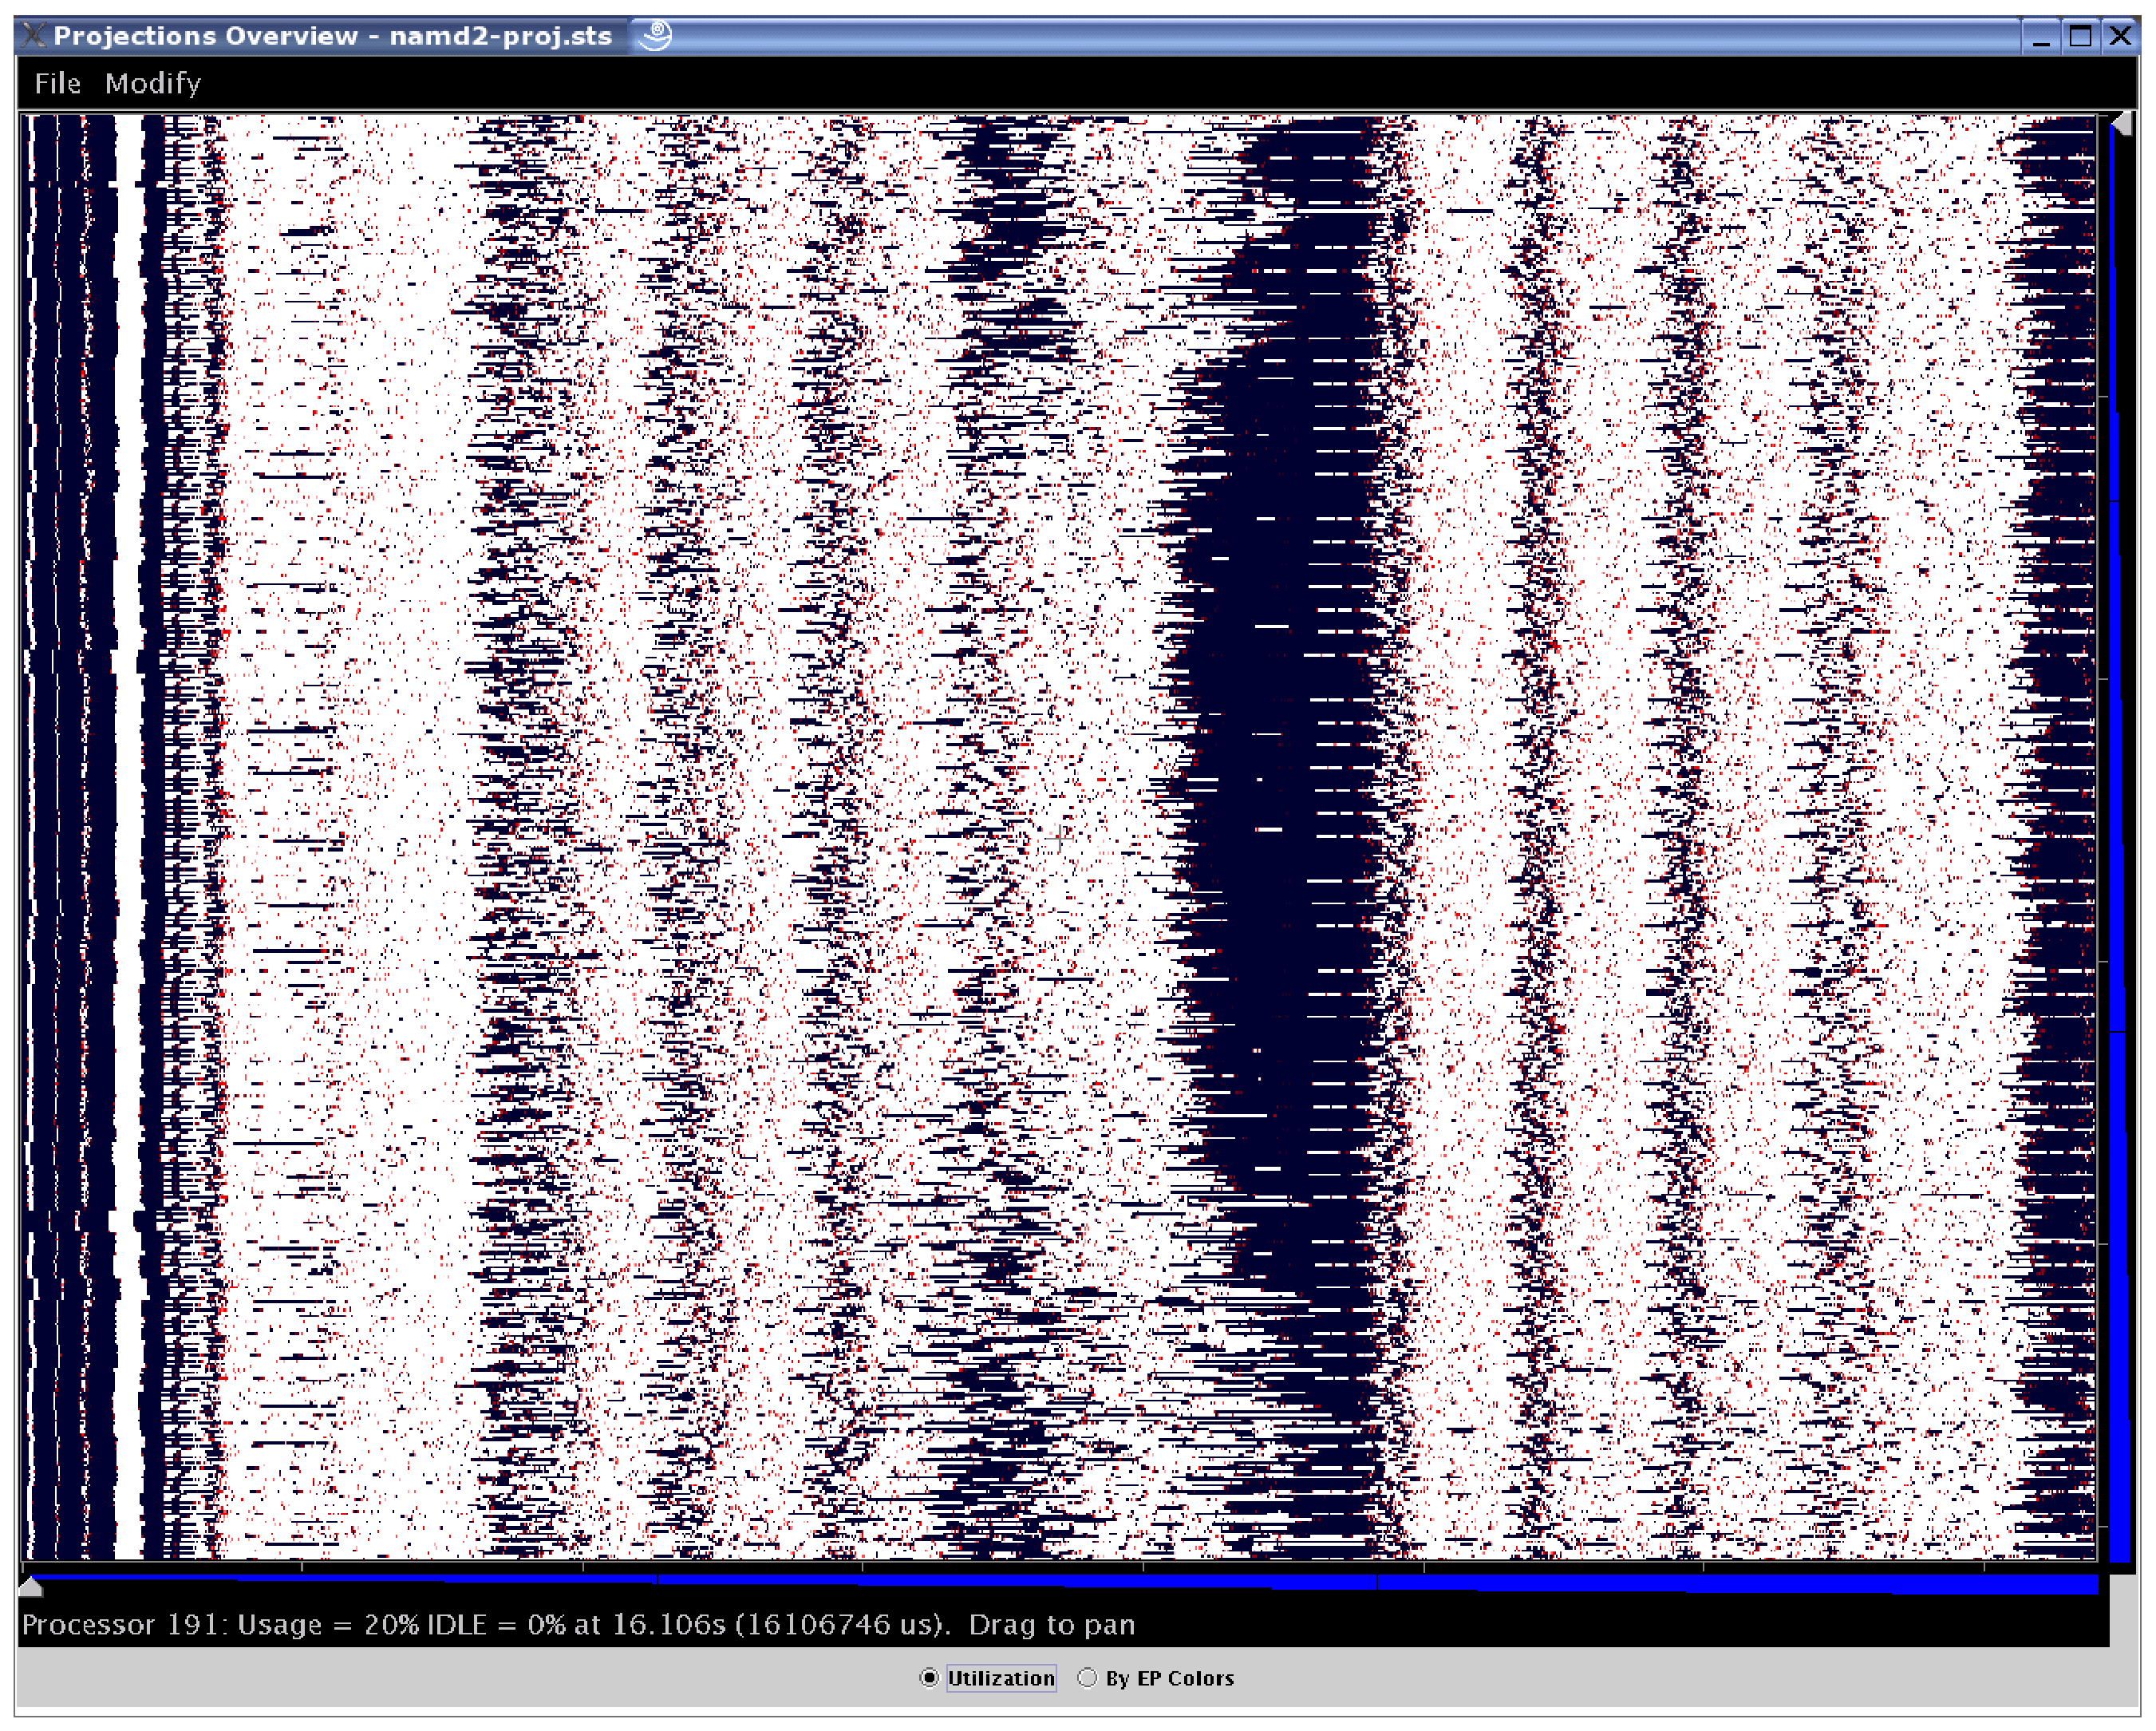
\includegraphics[width=3in]{fig/apoa1_512_overview}
    \label{overview}
  } 
  \subfigure[Overview with dominant Entry Method colors]{
    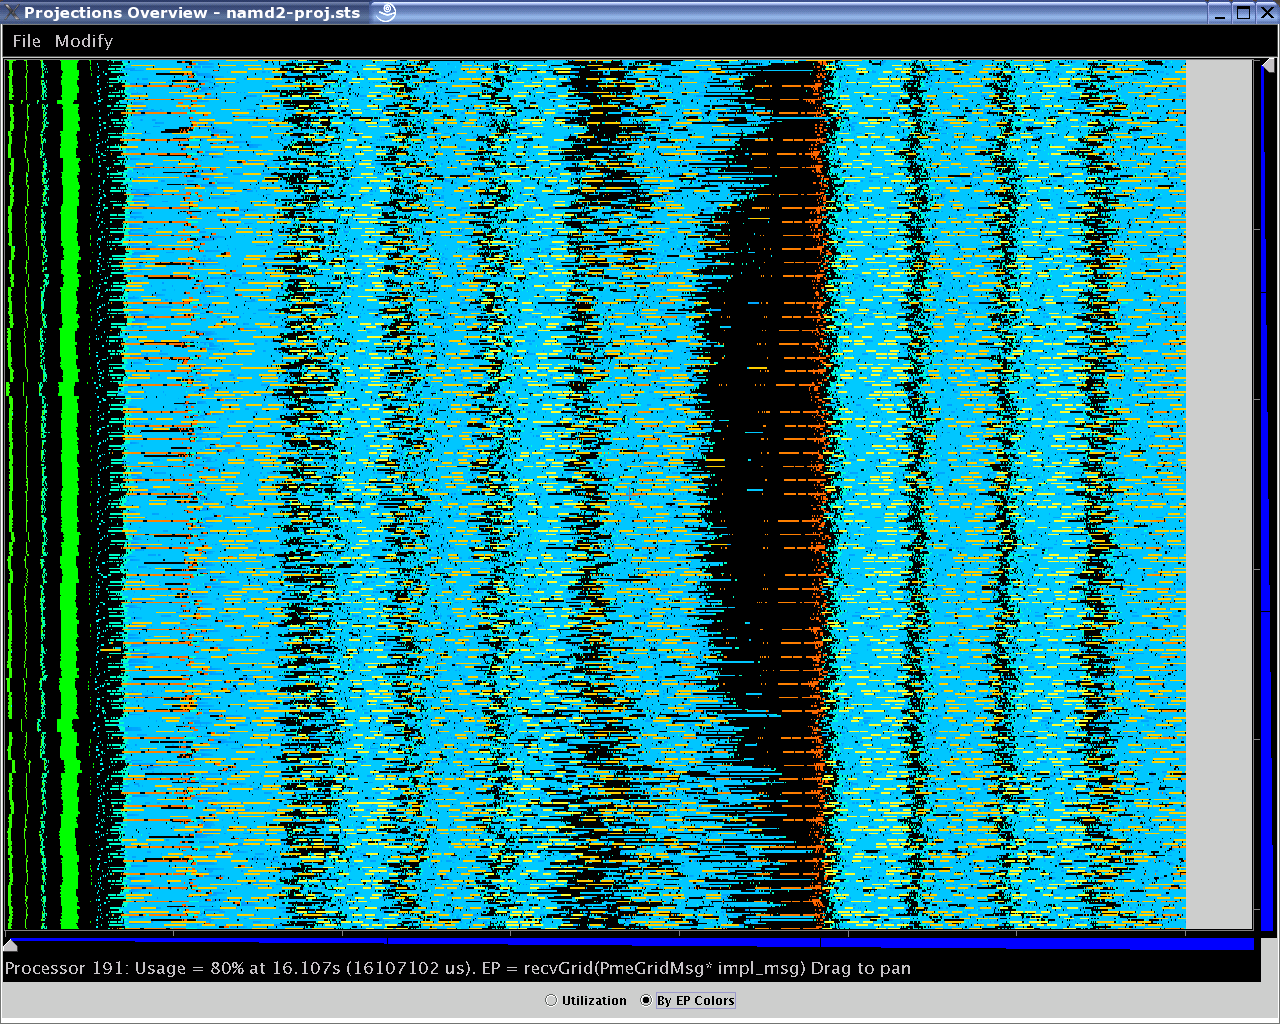
\includegraphics[width=3in]{fig/apoa1_512_overviewEPColored}
    \label{overview-ep}
  }
  \caption{Different Overview presentation forms.}
  \label{overview forms}
\end{figure}

%\begin{figure}[htb]
%\center
%\epsfig{figure=fig/overview.eps,height=4in}
%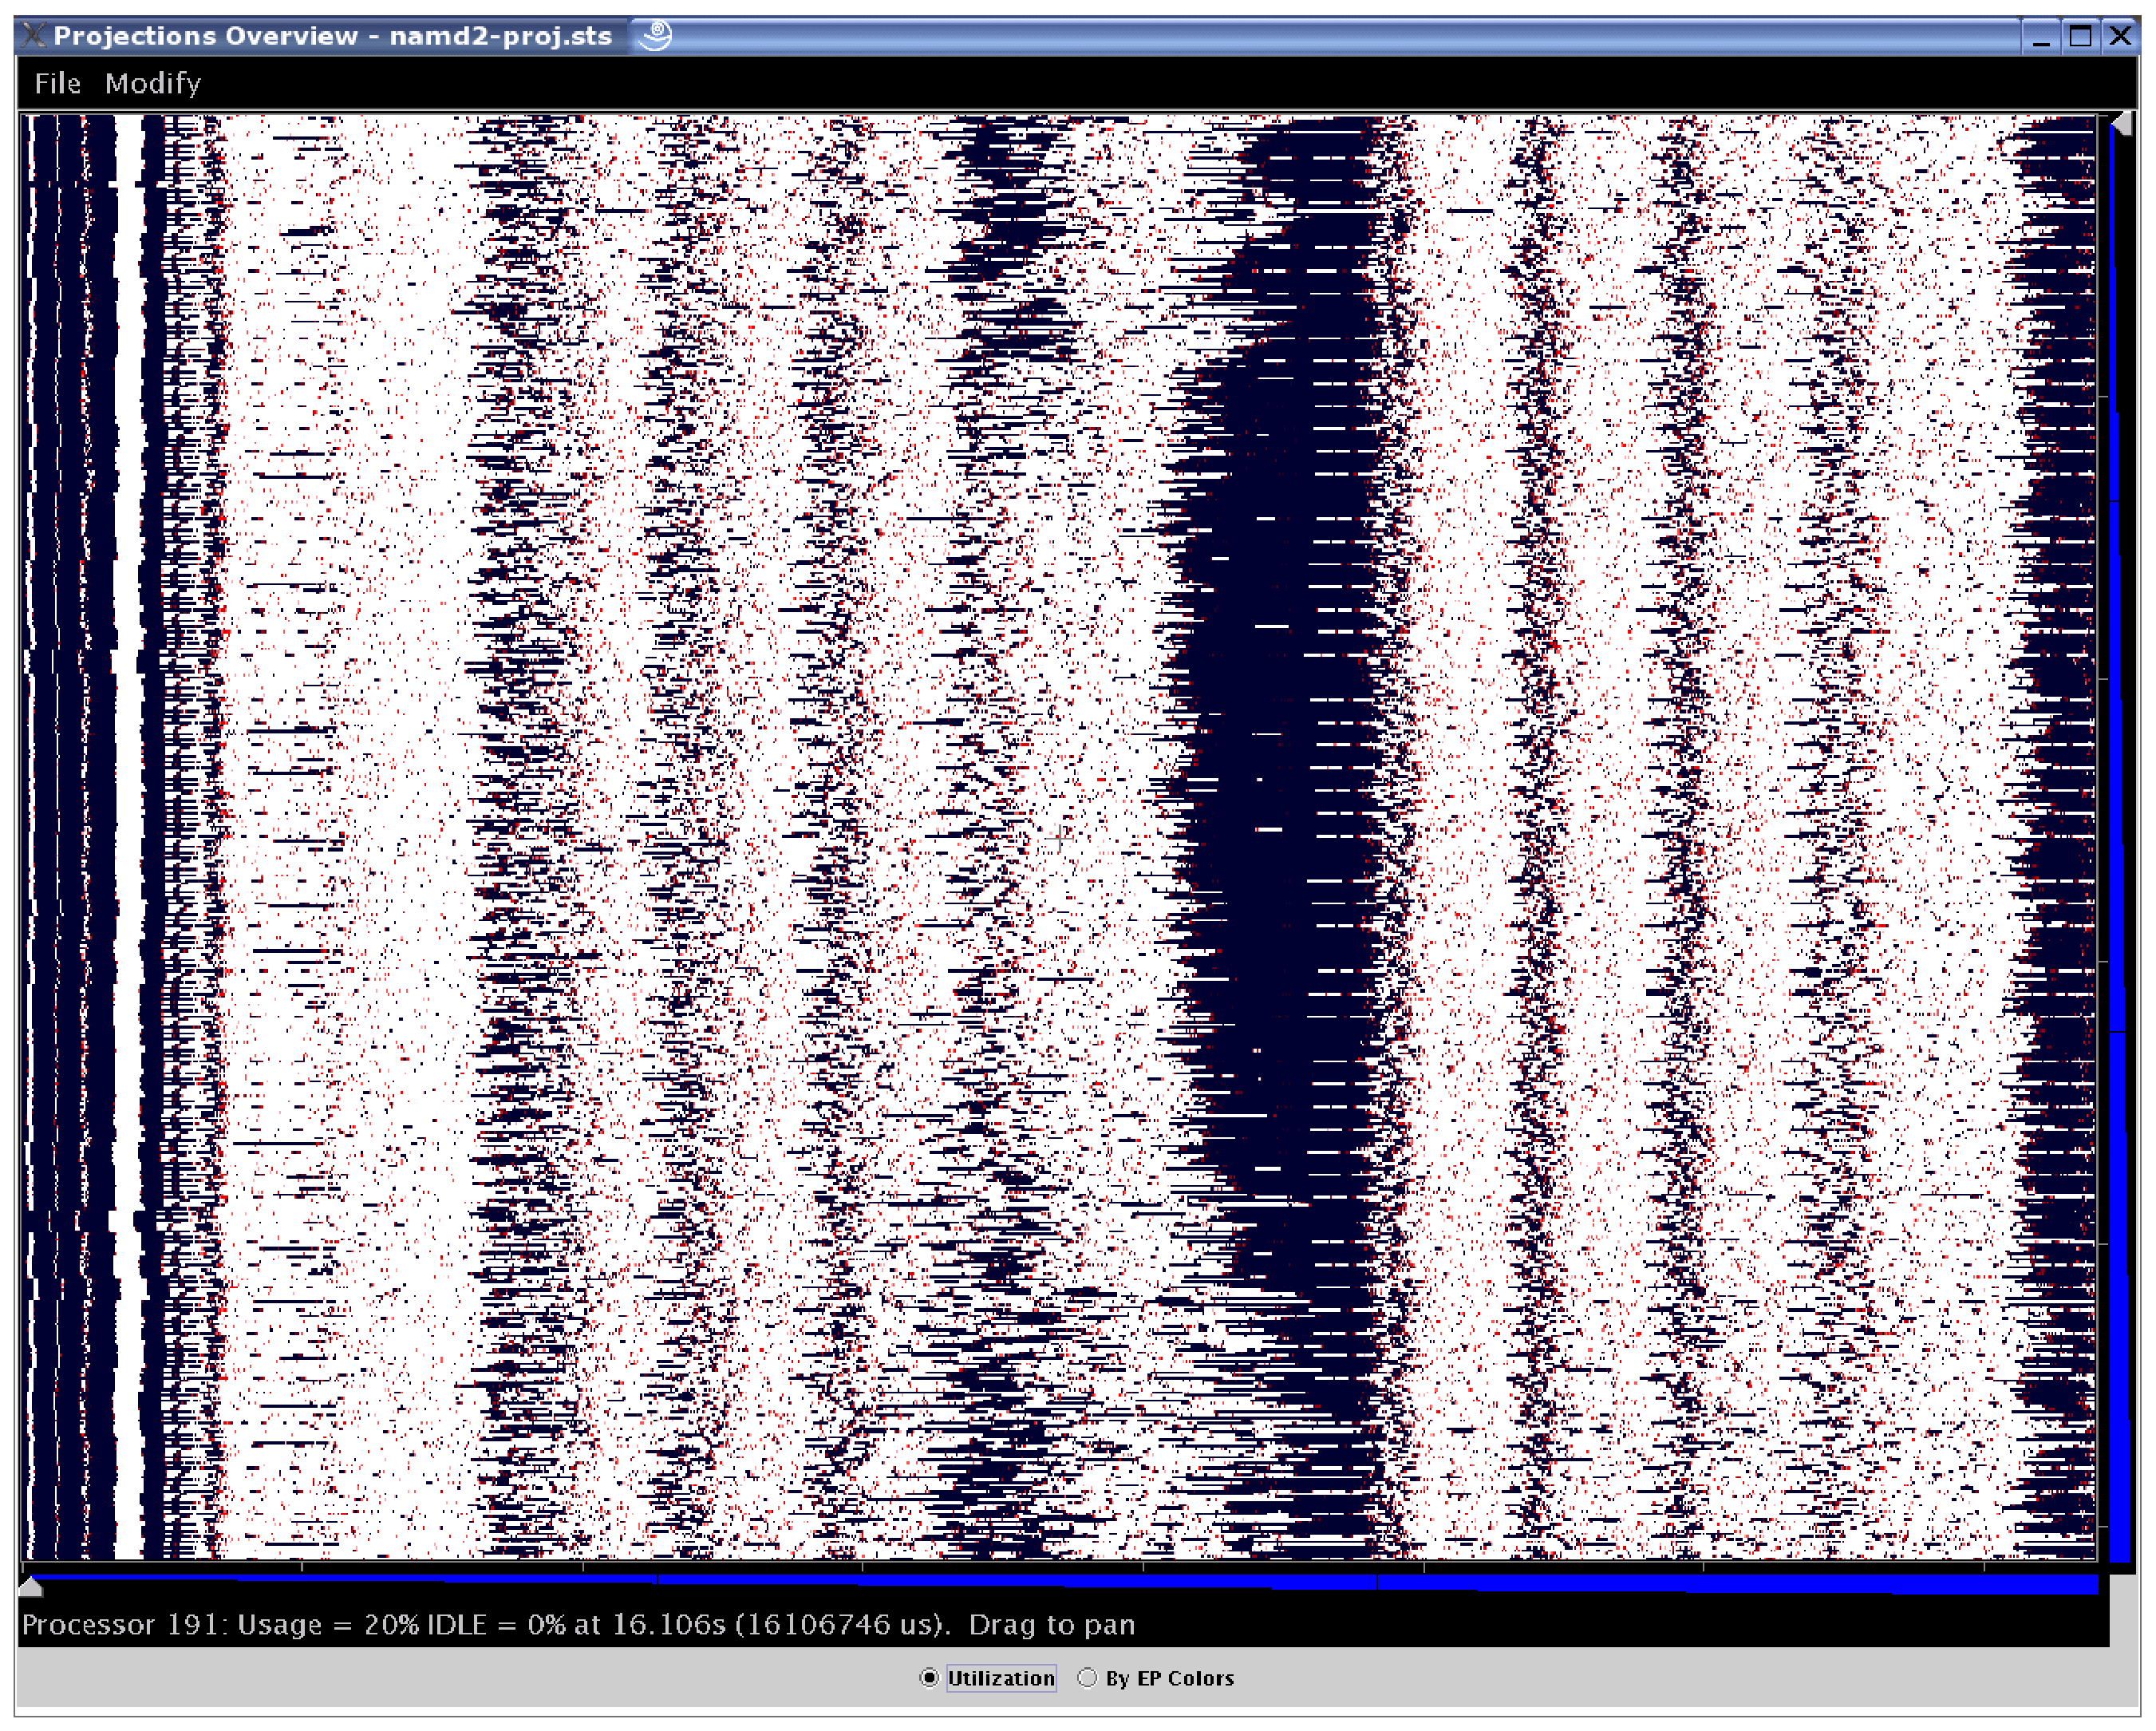
\includegraphics[width=4.0in]{fig/apoa1_512_overview}
%\caption{Overview}
%\label{overview}
%\end{figure}
%
%\begin{figure}[htb]
%\center
%\epsfig{figure=fig/overview.eps,height=4in}
%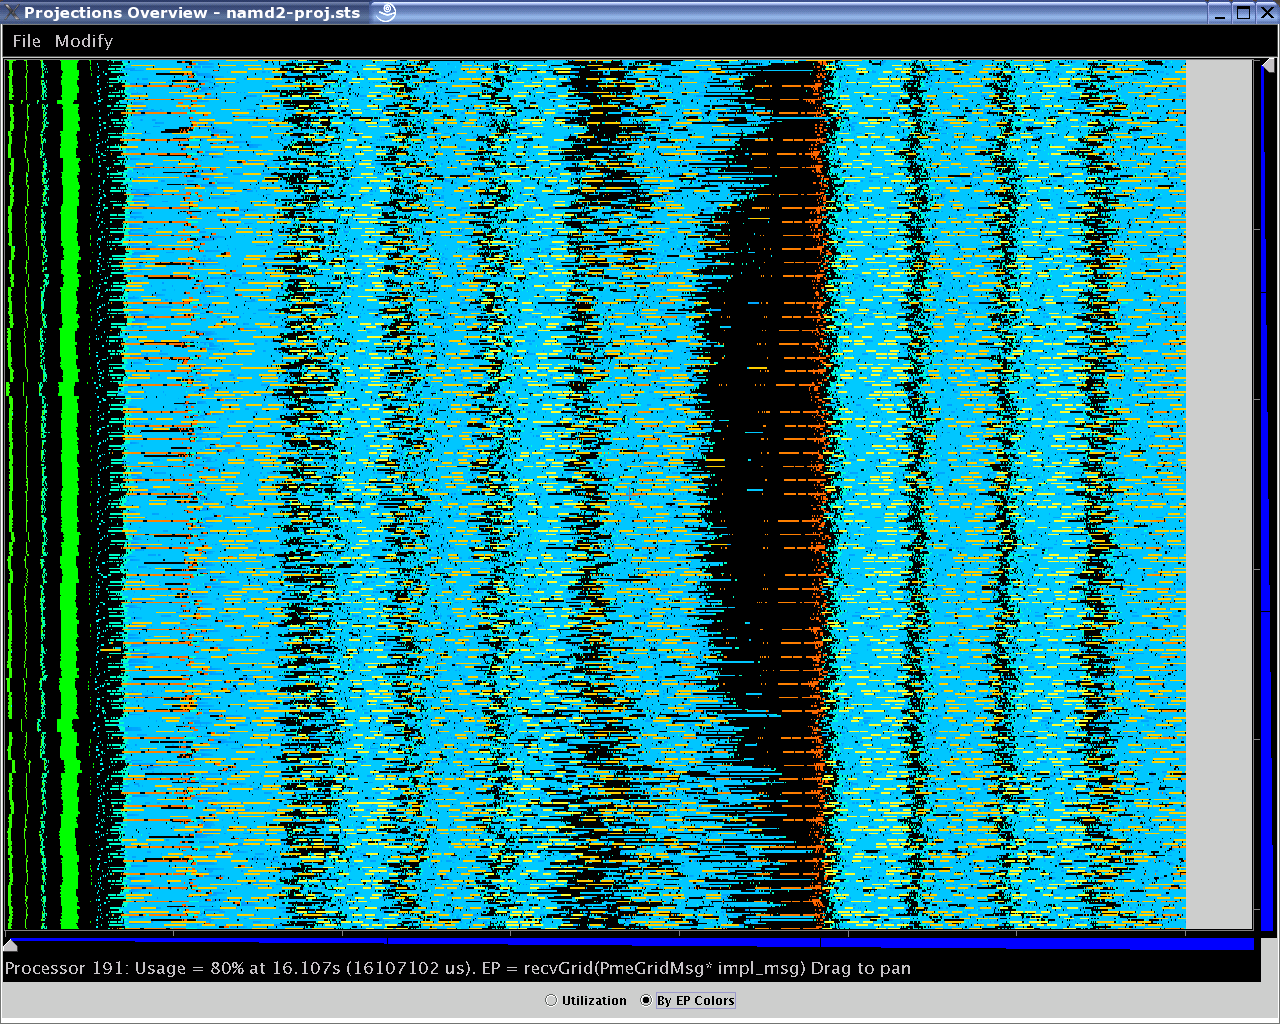
\includegraphics[width=4.0in]{fig/apoa1_512_overviewEPColored}
%\caption{Overview with dominant Entry Method colors}
%\label{overview-ep}
%\end{figure}

This tool provides support for the following menu options:

\begin{itemize}
\item {\bf File} provides 1 option: {\it Close} closes the current tool.
\item {\bf Modify} provides 1 option: {\it Set Range} reloads the
dialog box and allows the user to specify new parameters for rendering
new overview information.
\end{itemize}

The view currently hard codes the number of intervals to 7,000
independent of the time-range desired.

Each processor has a row of colored bars in the display, different
colors indicating different utilization at that time (White
representing 100% utilization, shades of red representing other
utilization (100% < utilization < 0%) and the background color
representing 0% utilization. Moving a mouse over the graph will invoke
a display of the processor usage of the specific processor at the
specific time in the status bar below the graph. Vertical and
horizontal zoom is enabled by two zooming bars to the right and lower
of the graph. Panning is possible by clicking on any part of the
display and dragging the mouse.

The ``by EP colors'' radio button provides more detail by replacing
the utilization colors with the colors of the most significant entry
method execution time in that time-interval on that processor
represented by the cells (as illustrated in figure
\ref{overview-ep}). 
%Be warned that this particular view is very likely
%a major visualization resource hog.

The Overview tool uses memory proportional to the number of processors
selected. If an out-of-memory error is encountered, try again by
skipping processors (e.g. {\tt 0-8191:2} instead of {\tt
0-8191}). This should show the general application structure almost as
well as using the full processor range.

\subsection{Animations}

This window (see figure \ref{animation}) animates the processor usage
over a specified range of time and a specified interval size.

The dialog box to load animation information is exactly the same as
that of the Graph tool (see section \ref{sec::graph view}).

\begin{figure}[htb]
\center
%\epsfig{figure=fig/animation.eps,height=3in}
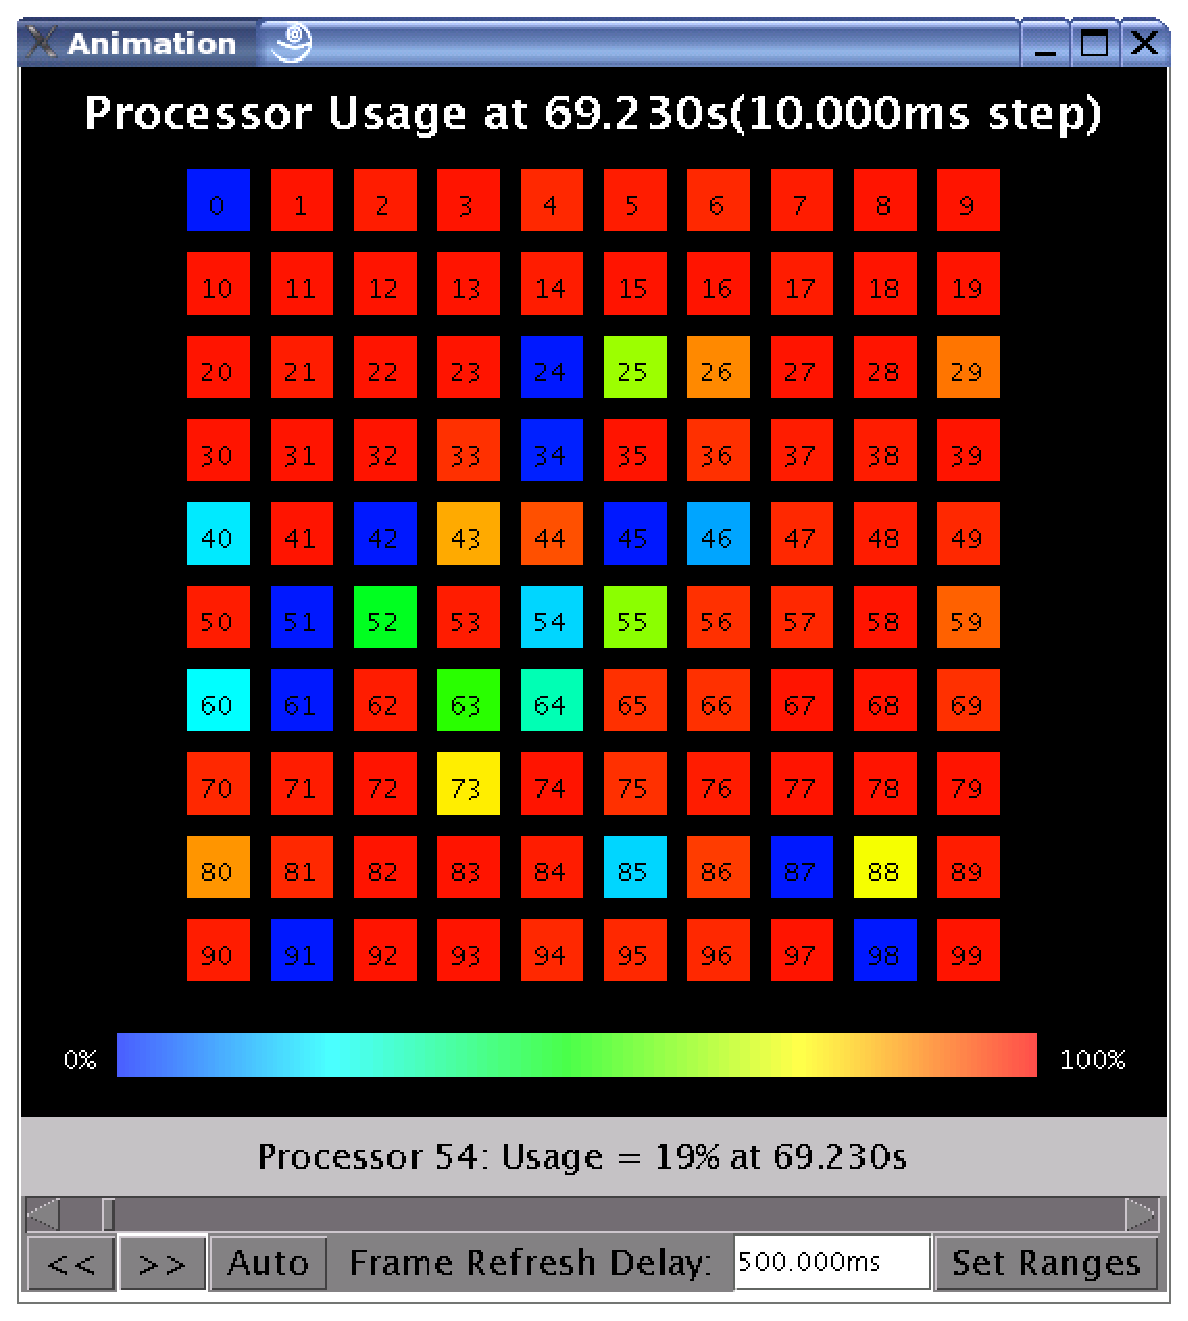
\includegraphics[width=2.5in]{fig/animation}
\caption{Animation View}
\label{animation}
\end{figure}

A color temperature bar serves as a legend for displaying different
processor utilization as the animation progresses. Each time interval
will have its data rendered as a frame. A frame displays in text on
the top of the display the currently represented execution time of the
application and what the size of an interval is.

Each selected processor is laid out in a 2-D plot as close to a square
as possible. The view employs a color temperature ranging from blue
(cool - low utilization) to bright red (hot - high utilization) to
represent utilization.

You may manually update the frames by using the ``$<<$'' or ``$>>$''
buttons to visualize the preceding or next frames respectively. The
``Auto'' button toggles automatic animation given the desired refresh
rate.

The ``Frame Refresh Delay'' field allows you to select the real time
delay between frames. It is a time-based field (see section
\ref{sec::misc} for special features in using time-based
fields).

The ``Set Ranges'' button allows you to set new parameters for this
view via the dialog box.

This view has no known performance issues.

\subsection{Time Profile Graph}

The Time Profile view (see figure \ref{time profile}) is a
visualization of the amount of time contributed by each entry method
summed across all processors and displayed by user-adjustable time
intervals.

Time Profile's dialog box is exactly the same as that of the Graph
tool (see section \ref{sec::graph view}).

\begin{figure}[htb]
\center
%\epsfig{figure=fig/timeprofile.eps,height=4in}
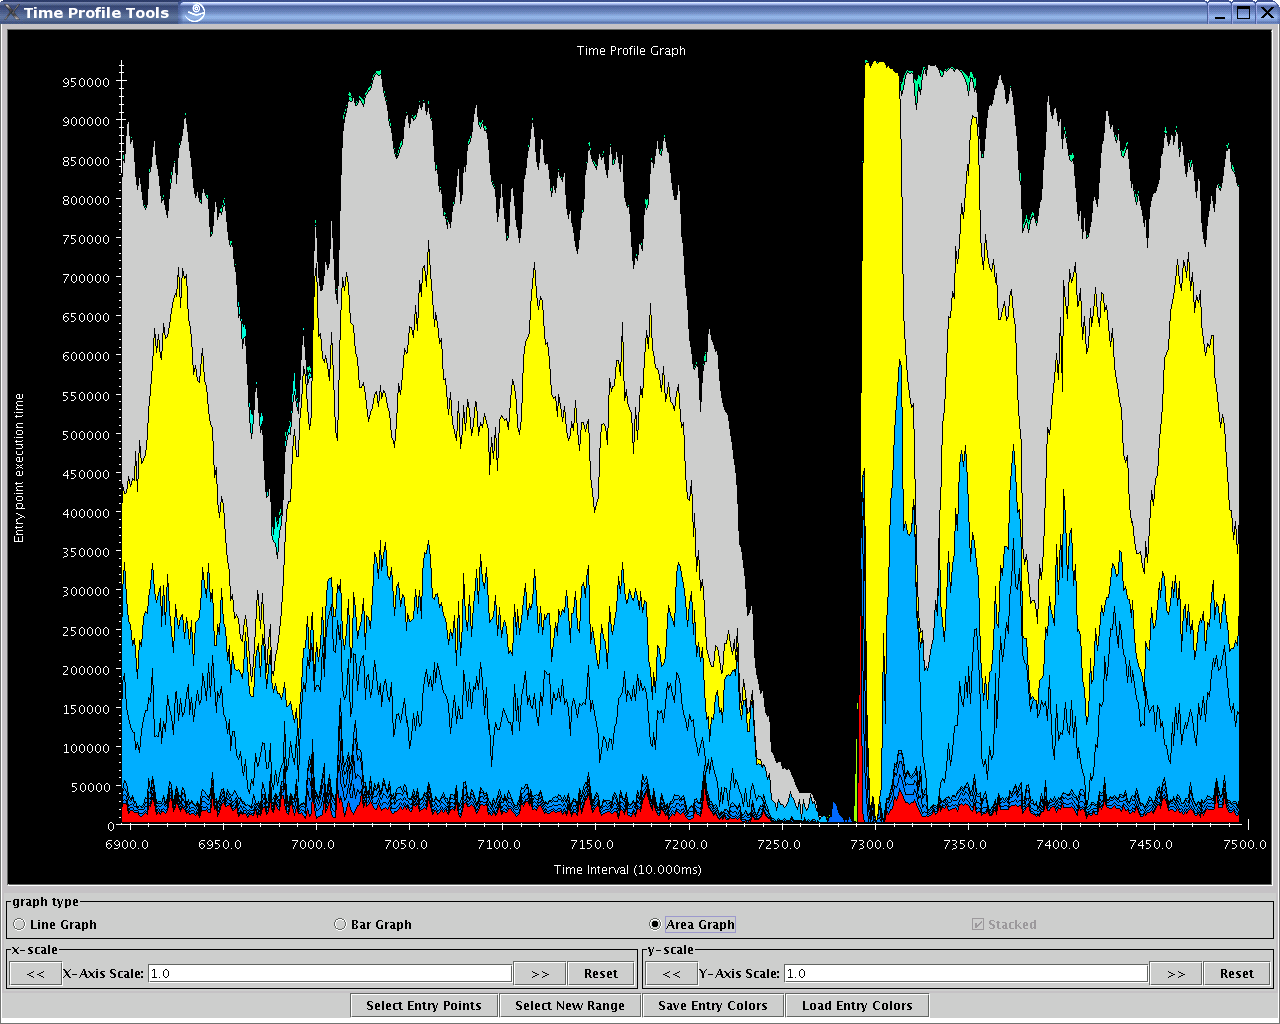
\includegraphics[width=4.0in]{fig/timeprofile}
\caption{Time Profile Graph View}
\label{time profile}
\end{figure}

Standard graph features can be employed for the main display of this
view (see section \ref{sec::misc}).

Under the tool options, one may:

\begin{itemize}
\item[-] Filter the set of entry methods to be displayed on the graph via
the ``Select Entry Points'' button. One may also modify the color set used
for the entry methods via this option.
\item[-] use the ``Select New Range'' button to reload the dialog box
for the tool and set new parameters for visualization (eg. different
time range, different set of processors or different interval sizes).
\item[-] store the current set of entry method colors to disk (to the
same directory where the trace logs are stored). This is done via the
``Save Entry Colors'' button.
\item[-] load the stored set of entry method colors (if it exists)
from disk (from the same directory where the trace logs are
stored). This is done via the ``Load Entry Colors'' button.
\end{itemize}

Time Profile also reacts to the presence of data about AMPI
functions (See section \ref{sec::AMPI functions}). When such data is
detected, an extra tabbed window displays a graph similar to entry
method profiles, but for AMPI functions only.

This tool's performance is tied to the number of intervals desired by
the user. We recommend that the user stick to visualizing 1,000
intervals or less.

\subsection{User Events Profile}

The User Events view is essentially a usage profile (See section
\ref{sec::usage profile}) of bracketed user events (if any) that were
recorded over a specified time range. The x-axis holds bars of data
associated with each processor while the y-axis represents the time
spent by each user event. Each user event is assigned a color.

\begin{figure}[htb]
\center
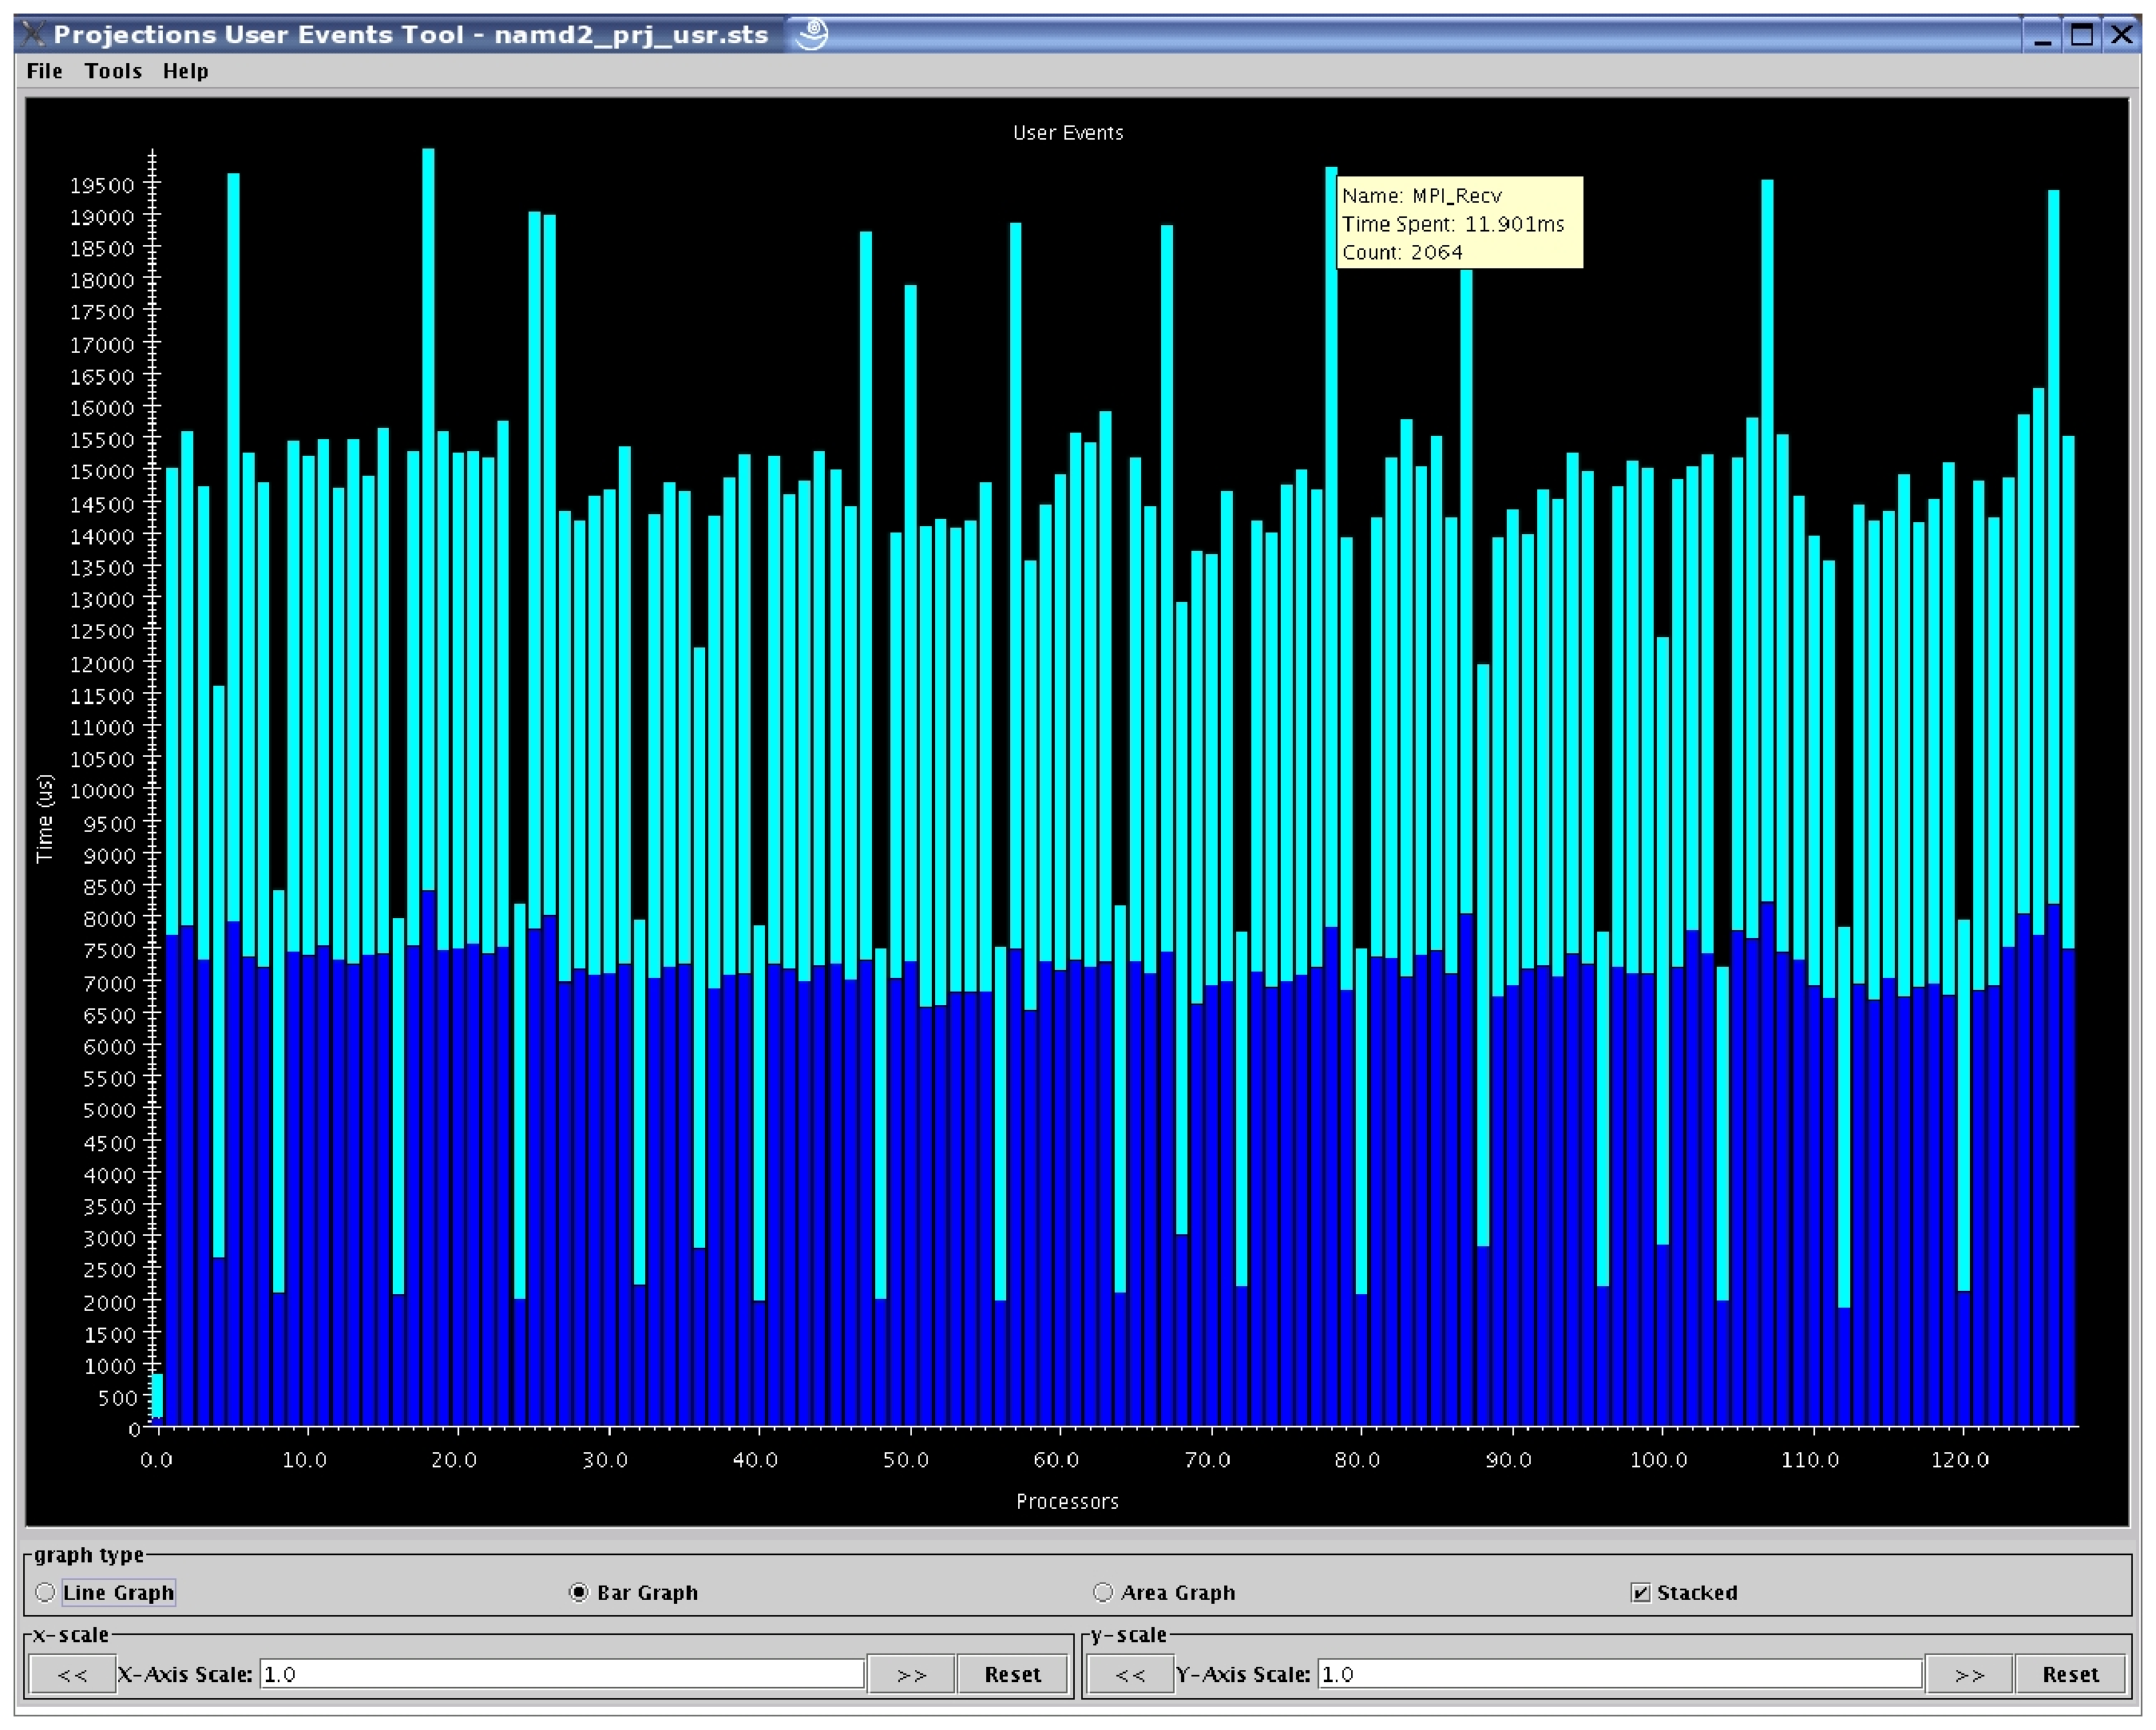
\includegraphics[width=4.0in]{fig/apoa1_128_userEventsView}
\caption{User Events Profile View}
\label{user event profile}
\end{figure}

It is important to note that user-events can be arbitrarily
nested. The view currently displays information based on raw data
without regard to the way the events are nested. Memory usage is
proportional to the number of processors to be displayed.

\subsection{Outlier Analysis}
\subsubsection{Outlier Analysis}
\label{sec::outlier}

For performance logs generated from large numbers of processors, it is
often difficult to view in detail the behavior of poorly behaved
processors. This view attempts to present information similar to usage
profile but only for processors whose behavior is ``extreme''.

\begin{figure}[htb]
\center
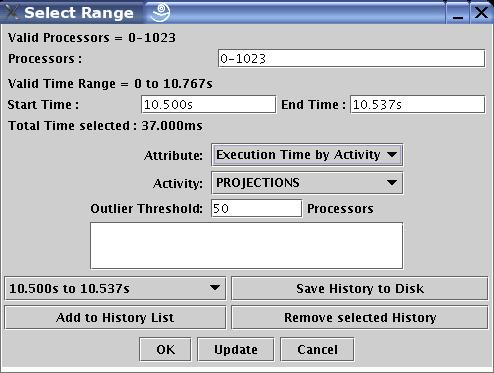
\includegraphics[width=4.0in]{fig/outlier_dialog}
\caption{Outlier Analysis Selection Dialog}
\label{outlier dialog}
\end{figure}

``Extreme'' processors are identified through the application of
heuristics specific to the attribute that analysts wish to study
applied to a specific activity type. You can specify the number of
``extreme'' processors are to be picked out by \projections{} by
filling the appropriate number in the field ``Outlier Threshold''. The
default is to pick 10\% of the total number of processors up to a cap
of 20. As an example, an analyst may wish to find ``extreme''
processors with respect to the idle time of normal \charmpp{} trace
events.

Figure \ref{outlier dialog} shows the choices available to this
tool. Specific to this view are two pull-down menus: {\em Attribute}
and {\em Activity}.

There are four {\em Activity} options:
\begin{enumerate}
\item The {\em Projections} activity type refer to the entry methods 
executed by the \charmpp{} runtime system.
\item The {\em User Events} activity type refer to records of events
as captured through {\tt traceUserEvent}-type calls described in
section \ref{sec::user events}.
\item The {\em Functions} activity type refer to the events captured
for AMPI functions through the functions described in section
\ref{sec::AMPI functions}.
%\item The {\em POSE} activity type refers to events captured for POSE
%parallel discrete event simulations through the interface described in
%section \ref{sec::POSE}.
\end{enumerate}

There are four {\em Attribute} options:
\begin{enumerate}
\item {\em Execution time by Activity} tells the tool to apply heuristics
based on the execution time of each instance of an activity occuring
within the specified time range.
\item {\em Idle time} tells the tool to apply a simple sort over all
processors on the least total idle time recorded. This will work only for
the {\em Projections} activity type.
\item {\em Msgs sent by Activity} tells the tool to apply heuristics
based on the number of messages sent over each instance of an
activity occuring within the specified time range. This option is
currently not implemented but is expected to work over all activity
types.
\item {\em Bytes sent by Activity} tells the tool to apply heuristics
based on the size (in bytes) of messages sent over each instance of an
activity occuring within the specified time range. This option is
currently not implemented but is expected to work over all activity
types.
\end{enumerate}

\begin{figure}[htb]
\center
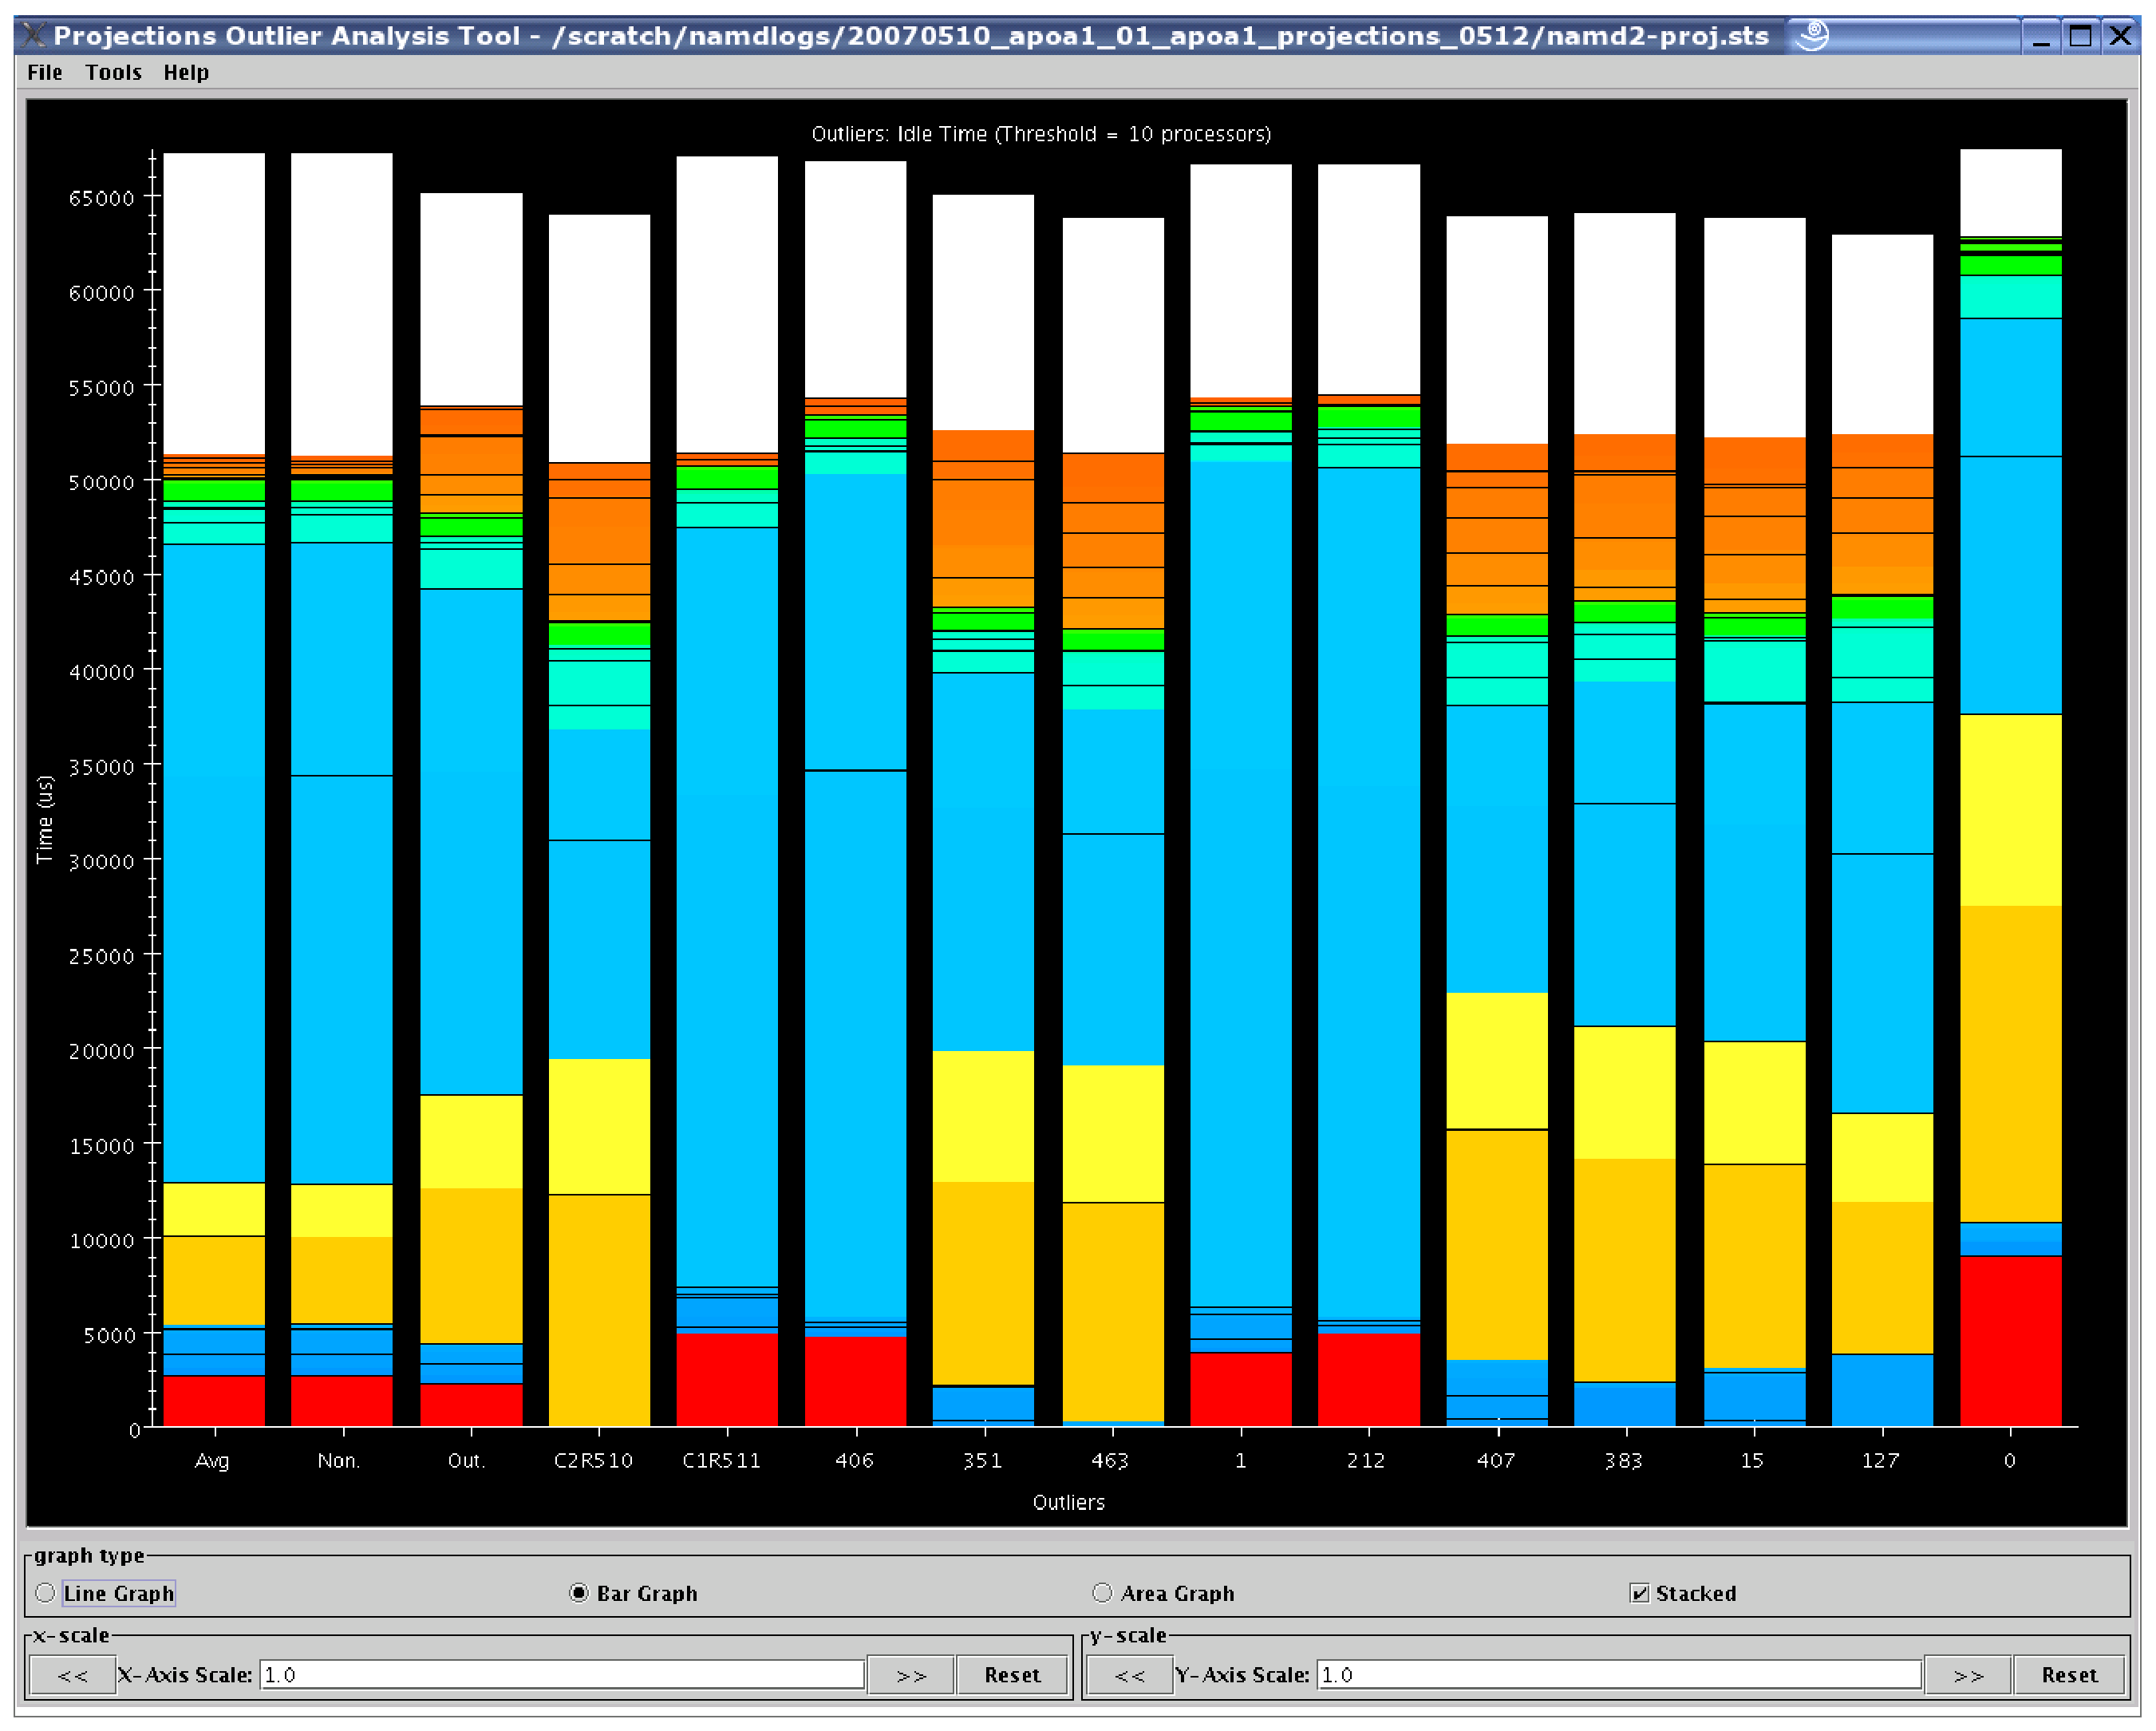
\includegraphics[width=4.0in]{fig/apoa1_512_outlierWithClusters}
\caption{Outlier Analysis View}
\label{outlier view}
\end{figure}

At the same time, a k-means clustering algorithm is applied to the
data to help identify processors with exemplar behavior that is
representative of each cluster (or equivalence class) identified by
the algorithm. You can control the value of k by filling in the
appropriate number in the field ``Number of Clusters''. The default
value is 5.

The result of applying the required heuristics to the appropriate {\em
attribute} and {\em activity} types results in a chart similar to
figure \ref{outlier view}. This is essentially a usage profile that
shows, over the user's selected time range, from left to right:

\begin{itemize}
\item A bar representing the global average of execution time of each
activity over all processors.
\item A bar representing the average activity profile of all
non-outlier (or non-extreme) processors.
\item A bar representing the average activity profile of all outlier
(or extreme) processors identified by the heuristics.
\item One bar representing the activity profile of the representative
processor from each cluster of processors identified by the application
of the k-means clustering algorithm.
\item One bar representing the activity profile of each identified
outlier processor, sorted in order of significance (rightmost processor
bar is the most significant).
\end{itemize}

The tool helps the user reduce the number of processor bars that must
be visually examined in order to identify candidates for more detailed
study. To further the cause of this goal, if the analyst has the {\em
timeline} view (see section \ref{sec::timeline view}) open, a
mouse-click on any of the processor activity profile bars (except for
group-averaged bars) will load that processor's detailed timeline
(over the time range specified in the timeline view) into the timeline
view itself.

%\begin{figure}[htb]
%\center
%\includegraphics[width=4.0in]{fig/outlier_dialogAttributes}
%\caption{Outlier Analysis Attributes available}
%\label{outlier attributes}
%\end{figure}

%\begin{figure}[htb]
%\center
%\includegraphics[width=4.0in]{fig/outlier_dialogActivities}
%\caption{Outlier Analysis Activity Types available}
%\label{outlier activities}
%\end{figure}



\subsection{ Online Live Analysis}
Projections provides a continuous performance monitoring tool - CCS streaming. 
Different from other tools discussed above, which are used to visualize post-mortem data, 
ccs streaming visualizes the running programs. In order to use it, the Charm++
program needs to be linked with \textbf{-tracemode utilization}.
The command line needs to include "++server ++server-port 2345". "2345" is 
the socket port number on server side.
In projections ccs streaming tool, the port number should be same with that on server side.


\subsection{Multirun Analysis}

\subsection{Function Tool}
\label{sec::function tool}
The Function Tool view presents a graph that is a usage profile (See
section \ref{sec::usage profile}) of AMPI function information. This
view allows the analyst to choose to display the time spent by each
function or the number of calls made over the selected time range.

In the case of AMPI functions, the events are properly nested. The
information displayed is currently that of {\em inclusive time}
(i.e. if function B's calls are nested within function A's, the time
spent in function B contribute to both function B's and function A's
displayed performance information). There are plans to implement the
presentation of AMPI function information based on {\em exclusive
time} (i.e. time within functions are computed by subtracting the
measured time spent minus the time spent by any calls to nested
functions).

%\subsection{POSE Analysis}

\subsection{AMPI Usage Profile}

The AMPI Usage Profile view presents a graph similar to Function
Tool's (See section \ref{sec::function tool}) with several
modifications:

\begin{enumerate}
\item In it's per-processor mode, displayed via the tabbed window
``Per Processor'', the information displayed includes the time spent
by other events outside of AMPI. This is displayed as a white bar
marked ``Others'' when moused-over. This allows the analyst to compare
the time spent by events within AMPI functions along with other
recorded events. In contrast, Function Tool shows only AMPI function
events.
\item In it's per-function mode, displayed via the tabbed window ``Per
Function'', the information is displayed with each bar on the x-axis
showing the percentage utilization for a different AMPI function.
\end{enumerate}


\subsubsection{NoiseMiner View}

The NoiseMiner view (see figure \ref{time profile}) displays statistics about abnormally long entry methods. Its purpose is to detect symptoms consistent with \textit{Operating System Interference} or \textit{Compuatational Noise}. The abnormal events are filtered and clustered across multiple dimensions to produce a concise summary. The view displays both the duration of the events as well as the periodicity at which they occur. Its dialog box is exactly the same as that of the Graph tool (see section \ref{sec::graph view}).

The tool uses stream mining techniques to produce its results by making only one pass through the input data while using a limited amount of memory. This allows NoiseMiner to be very fast and scalable. 

\begin{figure}[htb]
\center
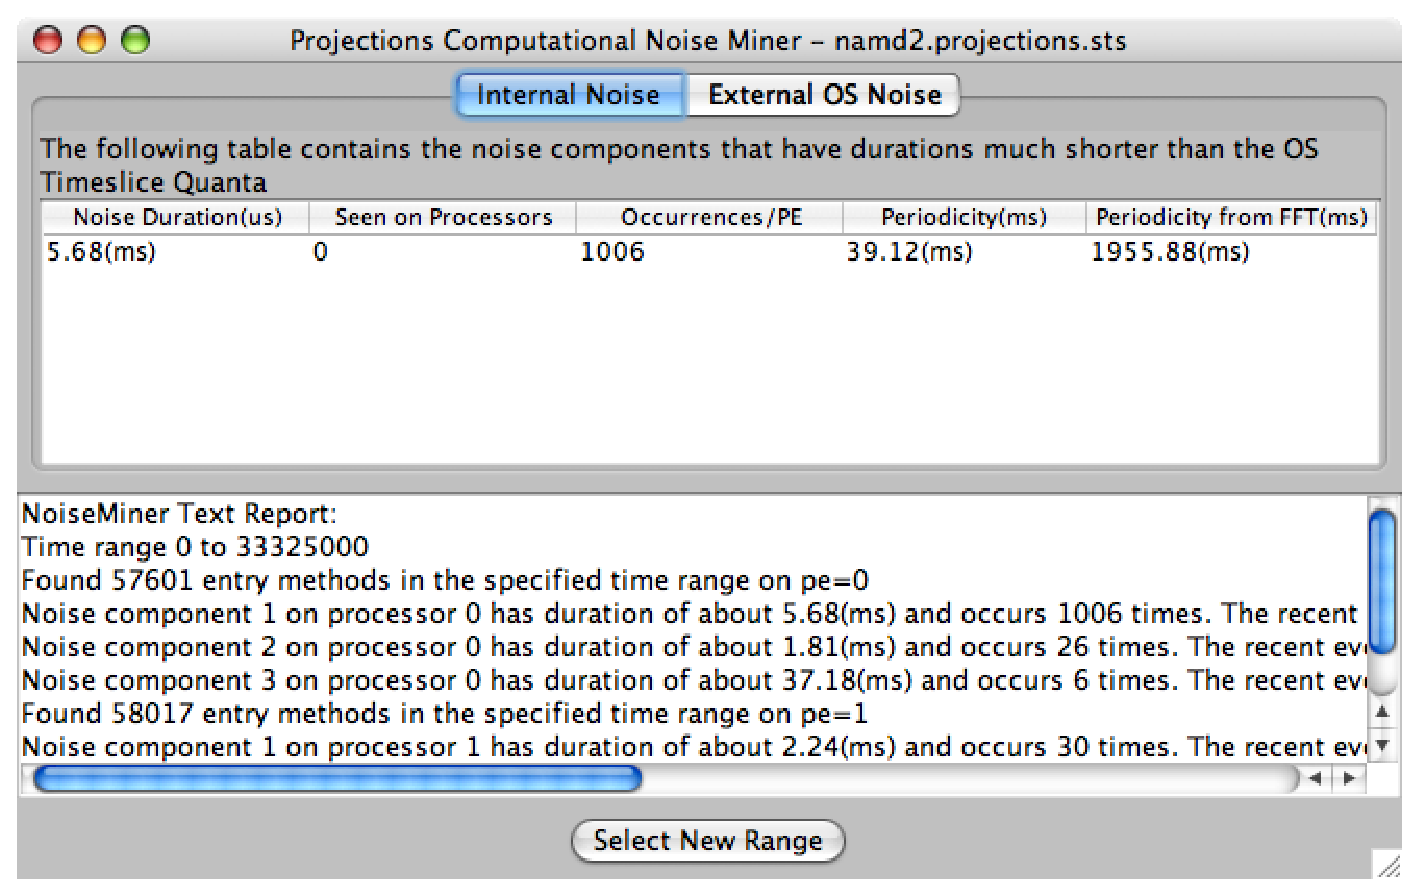
\includegraphics[width=4.0in]{fig/noiseminer}
\caption{NoiseMiner View displaying one \textit{Internal Noise} component of duration 5.68(ms) that occurred 1006 times during the run. This shows that there is likely some OS interference or Computational Noise problem occurring during the run. In this case, a faulty MPI implementation took an extra 5 ms to complete various calls which should have taken less than 0.1 ms.}
\label{noiseminer}
\end{figure}

NoiseMiner works by storing histograms of each entry method's duration. The histogram bins contain a window of recent occurrences as well as an average duration and count. After data stream has been parsed into the histogram bins, the histogram bins are clustered to determine the ``normal'' entry method duration. The histograms are then normalized by the ``normal'' duration so that they represent the abnormally stretched amounts for the entry methods. Then the histogram bins are clustered by duration and across processors. Any clusters that do not contribute much to the overall runtime are dropped. Finally each cluster is reported as shown in figure \ref{noiseminer}. The resulting clusters are displayed in one of two tabs: the \textit{Internal Noise} tab will list any events width periodicity significantly shorter than the OS time quantum which is currently hard-coded to 100ms while the \textit{External Noise} tab will list any events width periodicity close to or longer than the OS time quanta. A slightly more detailed text report is also provided in the bottom pane of the window for user's wishing to record the information for future reference.

\section{Miscellaneous features}
\label{sec::misc}

\subsection{Standard Graph Display Interface} 

A standard graph display (an example of which can be found with the
Main Summary Graph - figure \ref{mainwindow}) has the following
features:

\begin{itemize}
\item[-] {\bf Graph types} can be selected between ``Line Graph'' which
connects each data point with a colored line representing the
appropriate data entry. This information may be ``stacked'' or
``unstacked'' (controlled by the checkbox to the right). A ``stacked''
graph places one data point set (Y values) on top of another. An
``unstacked'' graph simply uses the data point's Y value to directly
determine the point's position; ``Bar Graph'' (the default) which
draws a colored bar for each data entry and the value of the data
point determines its height or starting position (depending on whether
the bar graph is ``stacked'' or ``unstacked''). A ``Bar Graph''
displayed in ``unstacked'' mode draws its bars in a tallest to
shortest order so that the large Y values do not cover over the small
Y values; ``Area Graph'' is similar to a ``Line Graph'' except that the
area under the lines for a particular Y data point set is also colored
by the data's appropriate color. ``Area Graph''s are always stacked.
\item[-] {\bf x-scale} allows the user to scale the X-Axis. This can be
done by directly entering a scaling factor in the text field (simple
numeric field - see below) or by using the ``$<<$'' or ``$>>$'' buttons
to increase or decrease the scale by 0.25 each time. The ``Reset'' button
changes the scale factor back to 1.0. A scrollbar automatically appears
if the scale factor causes the canvas to be larger than the window.
\item {\bf y-scale} allows the user to scale the Y-Axis. This functions 
similarly to the {\bf x-scale} feature where the buttons and fields are
concerned.
\end{itemize}

\subsection{Standard Dialog Features}

\begin{figure}[htb]
\center
%\epsfig{figure=fig/standard_dialog.eps,height=4in}
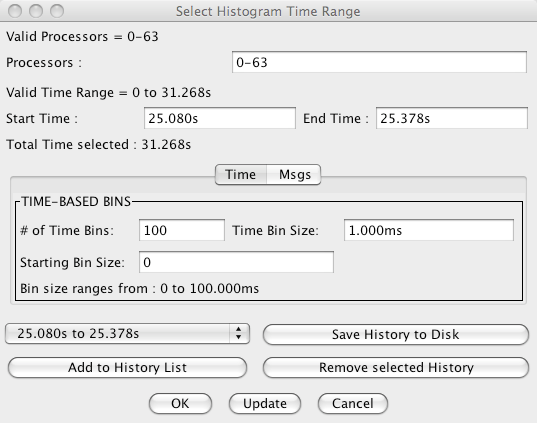
\includegraphics[width=2.5in]{fig/standard_dialog}
\caption{An example Dialog with standard fields}
\label{standard dialog}
\end{figure}

Figure \ref{standard dialog} shows a sample dialog box with standard
features. The following are standard features that can be employed in
such a dialog box:

\begin{itemize}
\item[-] {\bf Moving from field to field} via the tab key causes the
dialog box update the last field input by the user. It also performs a
consistency check. Whenever it finds an inconsistency, it will move
mouse focus onto the offending field, disabling the ``OK'' button so
as to force the user to fix the inconsistency. Examples of
inconsistency includes: input that violates a field's format; input
whose value violates constraints (eg. start time larger than end
time); or out-of-range stand-alone values.
\item[-] {\bf Available buttons} include ``OK'' which confirms the
user's choice of parameters. This button is only activated if the
dialog box considers the parameters' input to be
consistent. ``Update'' causes the dialog box to update the last field
input by the user and perform a consistency check. This is similar in
behavior to the user tabbing between fields. ``Cancel'' closes the
dialog box without modifying any parameters if the tool has already
been loaded or aborts the tool's load attempt otherwise.
\item[-] {\bf Parameter History} allows the user to quickly access
information for all tools for a set of frequently needed time
periods. An example of such a use is the desire by the analyst to view
a particular phase or timestep of a computation without having to
memorize or write on a piece of paper when exactly the phase or
timestep occurred.

It consists of a pull-down text box and 2 buttons. ``Add to History
List'' adds the current time range to the pull-down list to the left
of the button. The dialog box maintains up to 5 entries, replacing
older entries with newer ones. ``Remove Selected History'' removes the
currently selected entry in the history list. ``Save History to Disk''
stores current history information to the file ``ranges.hst'' in the
same directory where your logs are stored. Note that you will need
write access to that directory to successfully store history
information. A more flexible scheme is currently being developed and
will be released in a later version of \projections{}. Clicking on the
pull-down list allows the user to select one out of up to 5 possible
time ranges. You can do so by moving the mouse up or down the
list. Clicking on any one item changes the start and end times on the
dialog box.
\end{itemize}

\subsection{Data Fields}

Throughout \projections{} tools and dialog boxes (see sample figure
\ref{standard dialog}), data entry fields are provided. Unless
otherwise specified, these can be of the following standard field with
some format requirements:

\begin{itemize}
\item[-] {\bf Simple numeric fields}: An example can be found in
figure \ref{standard dialog} for ``Number of Bins:''. This field expects
a single number.
\item[-] {\bf Time-Based Field}: An example can be found in figure
\ref{standard dialog} for ``Start Time:''. This field expects a single
simple or floating point number followed by a time-scale modifier. The
following modifiers are supported: {\it none} - this is the default
and means the input number represents time in microseconds. A whole
number is expected; {\it The characters ``us''} - the input number
represents time in microseconds. A whole number is expected; {\it The
characters ``ms''} - the input number represents time in
milliseconds. This can be a whole number or floating point number; or
{\it The character ``s''} - the input number represents time in
seconds. This can be a whole number or floating point number.
\item[-] {\bf Processor-Based Field}: An example can be found in
figure \ref{standard dialog} for ``Processors:''. This field expects a
single whole number; a list of whole numbers; a range; or a mixed list
of whole numbers and ranges. Here are some examples which makes the
format clearer:

   eg: Want to see processors 1,3,5,7:  Enter {\tt 1,3,5,7}

   eg: Want to see processors 1,2,3,4:  Enter {\tt 1-4}

   eg: Want to see processors 1,2,3,7:  Enter {\tt 1-3,7}

   eg: Want to see processors 1,3,4,5,7,8: Enter {\tt 1,3-5,7-8}

Ranges also allow skip-factors. Here are some examples:

   eg: Want to see processors 3,6,9,12,15: Enter {\tt 3-15:3}

   eg: Want to see processors 1,3,6,9,11,14: Enter {\tt 1,3-9:3,11,14}

This feature is extremely flexible. It will normalize your input to a
canonical form, tolerating duplication of entries as well as
out-of-order entries (ie. {\tt 4,6,3} is the same as {\tt 3-4,6}).
\end{itemize}

\section{Known Issues}
\label{sec::known issues}

This section lists known issues and bugs with the \projections{}
framework that we have not resolved at this time.

\begin{itemize}
\item
\charmpp{} scheduler idle time is known to be incorrectly recorded on
the BG/L machine at IBM TJ Watson.
\item
End-of-Run analysis techniques (while tracing applications) are
currently known to hang for applications that make multiple calls to
traceBegin() and traceEnd() on the same processor through multiple
\charmpp{} objects.
\end{itemize}

\end{document}
